% Options for packages loaded elsewhere
\PassOptionsToPackage{unicode}{hyperref}
\PassOptionsToPackage{hyphens}{url}
\PassOptionsToPackage{dvipsnames,svgnames*,x11names*}{xcolor}
%
\documentclass[
  10pt,
  dvipsnames]{scrartcl}
\usepackage{amsmath,amssymb}
\usepackage{lmodern}
\usepackage{ifxetex,ifluatex}
\ifnum 0\ifxetex 1\fi\ifluatex 1\fi=0 % if pdftex
  \usepackage[T1]{fontenc}
  \usepackage[utf8]{inputenc}
  \usepackage{textcomp} % provide euro and other symbols
\else % if luatex or xetex
  \usepackage{unicode-math}
  \defaultfontfeatures{Scale=MatchLowercase}
  \defaultfontfeatures[\rmfamily]{Ligatures=TeX,Scale=1}
\fi
% Use upquote if available, for straight quotes in verbatim environments
\IfFileExists{upquote.sty}{\usepackage{upquote}}{}
\IfFileExists{microtype.sty}{% use microtype if available
  \usepackage[]{microtype}
  \UseMicrotypeSet[protrusion]{basicmath} % disable protrusion for tt fonts
}{}
\makeatletter
\@ifundefined{KOMAClassName}{% if non-KOMA class
  \IfFileExists{parskip.sty}{%
    \usepackage{parskip}
  }{% else
    \setlength{\parindent}{0pt}
    \setlength{\parskip}{6pt plus 2pt minus 1pt}}
}{% if KOMA class
  \KOMAoptions{parskip=half}}
\makeatother
\usepackage{xcolor}
\IfFileExists{xurl.sty}{\usepackage{xurl}}{} % add URL line breaks if available
\IfFileExists{bookmark.sty}{\usepackage{bookmark}}{\usepackage{hyperref}}
\hypersetup{
  pdftitle={Personal attacks decrease user activity in social networking platforms},
  colorlinks=true,
  linkcolor=Maroon,
  filecolor=Maroon,
  citecolor=Blue,
  urlcolor=blue,
  pdfcreator={LaTeX via pandoc}}
\urlstyle{same} % disable monospaced font for URLs
\usepackage{graphicx}
\makeatletter
\def\maxwidth{\ifdim\Gin@nat@width>\linewidth\linewidth\else\Gin@nat@width\fi}
\def\maxheight{\ifdim\Gin@nat@height>\textheight\textheight\else\Gin@nat@height\fi}
\makeatother
% Scale images if necessary, so that they will not overflow the page
% margins by default, and it is still possible to overwrite the defaults
% using explicit options in \includegraphics[width, height, ...]{}
\setkeys{Gin}{width=\maxwidth,height=\maxheight,keepaspectratio}
% Set default figure placement to htbp
\makeatletter
\def\fps@figure{htbp}
\makeatother
\setlength{\emergencystretch}{3em} % prevent overfull lines
\providecommand{\tightlist}{%
  \setlength{\itemsep}{0pt}\setlength{\parskip}{0pt}}
\setcounter{secnumdepth}{5}
%\documentclass{article}

% %packages
 \usepackage{booktabs}
 \usepackage[sort&compress]{natbib}
\usepackage{graphicx}
\usepackage{longtable}
\usepackage{ragged2e}
\usepackage{etex}
%\usepackage{yfonts}
\usepackage{marvosym}
\usepackage[notextcomp]{kpfonts}
\usepackage{nicefrac}
\newcommand*{\QED}{\hfill \footnotesize {\sc Q.e.d.}}
\usepackage{multicol} 
%\usepackage[textsize=footnotesize]{todonotes}
%\linespread{1.5}

\usepackage{float}

\usepackage{xcolor}

\setlength{\parindent}{10pt}
\setlength{\parskip}{1pt}


%language
%\usepackage{times}
\usepackage{mathptmx}
\usepackage[scaled=0.88]{helvet}

\usepackage{t1enc}
%\usepackage[utf8x]{inputenc}
%\usepackage[polish]{babel}
%\usepackage{polski}

\usepackage{subcaption}


%AMS
\usepackage{amsfonts}
\usepackage{amssymb}
\usepackage{amsthm}
\usepackage{amsmath}

%\usepackage{geometry}
 %\geometry{a4paper,left=35mm,top=20mm,}

%abbreviations
\newcommand{\ra}{\rangle}
\newcommand{\la}{\langle}
\newcommand{\n}{\neg}
\newcommand{\et}{\wedge}
\newcommand{\jt}{\rightarrow}
\newcommand{\ko}[1]{\forall  #1\,}
\newcommand{\ro}{\leftrightarrow}
\newcommand{\exi}[1]{\exists\, {_{#1}}}
\newcommand{\pr}{\mathsf{P}}
\newcommand{\odds}{\mathsf{Odds}}
\newcommand{\ind}{\mathsf{Ind}}
\newcommand{\nf}[2]{\nicefrac{#1\,}{#2}}
\newcommand{\R}[1]{\texttt{#1}}

\newtheorem{q}{\color{blue}Question}


%% Rafal's stuff
\usepackage[margin=1.5in,top=1in]{geometry}
\usepackage[textsize=scriptsize, textwidth = 3cm]{todonotes}
% This is my own comment shading, keep \todo for general stuff, feel free to define your own separate comment colors (usually useful if you use margin comments at tall) For instance, I defined one for Patrycja
\newcommand{\rt}[1]{\todo[color = orange!40]{#1}}
\newcommand{\pt}[1]{\todo[color = blue!40]{#1}}




\newtheorem*{reply*}{Reply}
\usepackage{enumitem}
\newcommand{\question}[1]{\begin{enumerate}[resume,leftmargin=0cm,labelsep=0cm,align=left]
\item #1
\end{enumerate}}

\usepackage{float}

% \setbeamertemplate{blocks}[rounded][shadow=true]
% \setbeamertemplate{itemize items}[ball]
% \AtBeginPart{}
% \AtBeginSection{}
% \AtBeginSubsection{}
% \AtBeginSubsubsection{}
% \setlength{\emergencystretch}{0em}
% \setlength{\parskip}{0pt}






\usepackage{booktabs}
\usepackage{longtable}
\usepackage{array}
\usepackage{multirow}
\usepackage{wrapfig}
\usepackage{float}
\usepackage{colortbl}
\usepackage{pdflscape}
\usepackage{tabu}
\usepackage{threeparttable}
\usepackage{threeparttablex}
\usepackage[normalem]{ulem}
\usepackage{makecell}
\usepackage{xcolor}
\ifluatex
  \usepackage{selnolig}  % disable illegal ligatures
\fi
\newlength{\cslhangindent}
\setlength{\cslhangindent}{1.5em}
\newlength{\csllabelwidth}
\setlength{\csllabelwidth}{3em}
\newenvironment{CSLReferences}[2] % #1 hanging-ident, #2 entry spacing
 {% don't indent paragraphs
  \setlength{\parindent}{0pt}
  % turn on hanging indent if param 1 is 1
  \ifodd #1 \everypar{\setlength{\hangindent}{\cslhangindent}}\ignorespaces\fi
  % set entry spacing
  \ifnum #2 > 0
  \setlength{\parskip}{#2\baselineskip}
  \fi
 }%
 {}
\usepackage{calc}
\newcommand{\CSLBlock}[1]{#1\hfill\break}
\newcommand{\CSLLeftMargin}[1]{\parbox[t]{\csllabelwidth}{#1}}
\newcommand{\CSLRightInline}[1]{\parbox[t]{\linewidth - \csllabelwidth}{#1}\break}
\newcommand{\CSLIndent}[1]{\hspace{\cslhangindent}#1}

\title{Personal attacks decrease user activity in social networking
platforms}
\author{}
\date{\vspace{-2.5em}}

\begin{document}
\maketitle

\vspace{-2mm}

\begin{abstract}
\noindent \textbf{Abstract.} 
We conduct a large scale data-driven analysis of the effects of online personal attacks on social media user activity. First, we perform a thorough overview of the literature on the influence of social media on user behavior, especially on the impact that negative and aggressive behaviors, such as harassment and cyberbullying, have on users’ engagement in online media platforms. The majority of previous research were  small-scale self-reported studies, which is their limitation. This motivates our data-driven study. We perform a large-scale analysis of messages from Reddit, a discussion website, for a period of two weeks, involving 182,528 posts or comments to posts by 148,317 users. To efficiently collect and analyze the data we apply a high-precision personal attack detection technology. We analyze the obtained data from three perspectives: (i) classical statistical methods, (ii) Bayesian estimation, and (iii) model-theoretic analysis. The three perspectives agree: personal attacks decrease the victims’ activity.
The results can be interpreted as an important signal to social media platforms and policy makers that leaving personal attacks unmoderated is quite likely to disengage the users and in effect depopulate the platform. On the other hand, application of cyberviolence detection technology in combination with various mitigation techniques could improve and strengthen the user community. As more of our lives is taking place online, keeping the virtual space inclusive for all users becomes an important problem which online media platforms need to face.


\vspace{4mm}


\noindent \textbf{Keywords:} verbal aggression online, personal attacks, social media, artificial intelligence, online engagement



\vspace{4mm}


\noindent \textbf{Significance.} Despite many efforts put into researching and preventing online aggression, it is still commonplace in cyber-encounters. Experiencing cyberbullying and harassment has been shown to lead to depression, feeling of hopelessness, and social media fatigue. People who experienced online harassment also reported disengagement and stopping using the services in which undesirable behavior occurred. Unfortunately, the existing literature and nearly whole body of research mostly studies the effects of verbal aggression on well-being relying only on self-reported data. Therefore it is often unclear if being subject to verbal aggression extends its effects on the behavioral level beyond the self-reported effects. We observe,  using a large-scale data-driven analysis, that experiencing verbal aggression online in the form of personal attacks indeed substantially decreases the victims’ activity.

\vspace{2mm}


\noindent \textbf{Disclaimer.} During the course of the study, we have utilized content that is publicly available on \textsf{Reddit.com} and can be accessed via the \textsf{Reddit} API or other similar technologies. This study was not  interventional research. Moreover,  although Reddit usernames are anonymous and usually do not display any personal information, we have additionally anonymized each one of them.  For these reasons, no informed consent was required (following point 8.05 of the \emph{Ethical Principles of Psychologists and Code of Conduct} of the American Psychological Association).\footnote{\textbf{Interests and authorship Disclaimer.}   \textsf{Samurai Labs} contributed 3000 PLN to the funding of this research. \textsf{Samurai Labs} prepared the raw data and results of personal attack recognition, and provided the humanpower to manually check which of 540 outliers  (even after the initial filtering out of bots) were bots. Some computing power was provided by National Science Center research grant number 2016/22/E/HS1/00304. Study design, \textsf{R} code, statistical analyses, their explanation and visualizations are due to Rafal Urbaniak (who has no interest in results going one way or the other, and no incentives related to any specific outcome were involved), theoretical discussion and further editorial work on the manuscript are  joint effort. Full .Rmd file with analysis code and anonymized datasets is available at \href{https://rfl-urbaniak.github.io/redditAttacks/}{https://rfl-urbaniak.github.io/redditAttacks/}.}
\normalsize



\thispagestyle{empty}

\end{abstract}

\section{Introduction}
\label{intro}

Recent decade brought an exponential growth of social networking
services (SNS) and associated with them social media platforms
(Ortiz-Ospina, 2019; Sheth, 2020), with
Facebook\footnote{\url{https://www.facebook.com/}} closing in on 2.85
billion users (one third of world population),
YouTube\footnote{\url{https://www.youtube.com/}} on close to 2 billion,
with smaller scale platforms such as
Twitter\footnote{\url{https://www.twitter.com/}} and
Reddit\footnote{\url{https://www.reddit.com/}} converging on around 350
million and over 430 million respectively (equivalent to the entire
population of the United States of America).

At the same time social media have witnessed an over ten
percentage-point drop in growth rate between 2012 and
2018,\footnote{\url{https://www.searchenginejournal.com/growth-social-media-v-3-0-infographic/}}
which suggests that the market is reaching over-satiation (Andersen,
2001) and most social media platforms will struggle for sustainable
growth. This leads to a shift from quantity-based to quality-based
growth policy, meaning that most social networking platforms will need
to focus not on how many new users to invite, but rather on how to keep
the existing users from leaving the platform and at the same time keep
them actively engaged.

One problem growing within the SNS that seriously hinders user
engagement is cyberbullying and various forms of Internet harassment
(Ptaszynski \& Masui, 2018). The global increase of the numbers of
Internet harassment cases has been related to the perceived anonymity
and thus the sense of impunity in users (Barlett, 2015; Barlett,
Gentile, \& Chew, 2016).

One of the most crude and common forms of cyberbullying are directed
personal attacks. In a typical personal attack user-attacker directly
verbally attacks user-victim with a harmful comment, or a set of harmful
comments, often based on a made-up excuse (e.g.~the victim expressed an
unpopular opinion). Often the attack not only remains unrestrained, but
also it escalates when other users join on either or both sides, causing
a wider distress not only to the victim, but also to a larger group of
users.

To specify the scale of this distress we study to what extent personal
attacks change the dynamics of user engagement in social media. First,
we present a thorough overview of the literature on how social networks
are affected by negative and destructive behavior and how this could be
mitigated by positive reactions. The literature suggests the hypothesis
that aggressive and generally abusive behaviors negatively influence
user engagement and therefore general user activity. To quantitatively
assess this hypothesis, we performed a large scale user activity
analysis on Reddit and drew a number of conclusions useful for SNS
moderators and policy makers.

The paper is organized as follows. Section \ref{literaturereview}
presents our review of the research on (1) factors influencing user
behavior in social media in general, (2) specific effects of online
harassment on user behavior, and in particular (3) factors that
influence users' continuous participation in SNS. Next, in Section
\ref{technology} we describe the technology we applied, which is both in
line with general accounts of personal attacks present in psychology,
and feasible from the technological point of view, and argue that the
technology is sufficiently precise for the current study. Section
\ref{quantanalysis} contains an in-depth large-scale analysis of Reddit
messages and personal attacks with the help of the technology provided
by \href{https://www.samurailabs.ai/}{\textsf{Samurai Labs}}. We expand
on the findings and discuss their more general meaning and importance,
as well as limitations of this study in Section \ref{discussion}.
Finally, we conclude the paper and indicate further paths to explore.

\section{Literature Review}
\label{literaturereview}

\subsection{The influence of  social media}

Even since the beginning of the social media popularity burst, studies
have indicated that participation in SNS influences the users'
well-being and social self-esteem, especially in adolescents.
Valkenburg, Peter, \& Schouten (2006), in a small initial survey study
(881 users) among young users (10-19 yo.) on a popular Dutch SNS called
CU2, already noticed that especially (1) the frequency and (2) the tone
(positive vs.~negative) of the feedback they received had a significant
(and correspondingly positive or negative) impact on the well-being and
social self-esteem of the users.

Although SNS have the potential to improve the users' lives, other
studies link frequent social media use, especially the one leading to
addiction, to various mental health problems, including low self esteem,
anxiety and depression (Beran \& Li, 2005; Campbell, Spears, Slee,
Butler, \& Kift, 2012; Hinduja \& Patchin, 2008; Woods \& Scott, 2016),
with similar results obtained all over the world, from the UK (Kelly,
Zilanawala, Booker, \& Sacker, 2018), Turkey (Kircaburun, 2016), to
Japan (Kitazawa et al., 2018), and Poland (Pyżalski, Zdrodowska,
Tomczyk, \& Abramczuk, 2019).

Culpepper (2020) recently studied the relationship between social media
use in youth and symptoms of depression and anxiety. The research
concluded that the amount of time spent on social media and symptoms of
depression were strongly correlated, although not that strong
correlation was found between the amount of time spent on social media
and the symptoms of anxiety. This suggests that some factors of the
social media use might cause the increase of such emotions associated
with depression as sadness, or powerlessness.

More detailed studies in this matter link the use of social media to the
feeling of \textit{fatigue}, defined as a self-regulated and subjective
feeling of tiredness that results from using certain SNS platforms.
Especially Malik, Dhir, Kaur, \& Johri (2020) investigated whether
different aspects of social media use (e.g., online privacy concerns,
social comparisons, self-disclosure, intensity of social media use and
FOMO, or the \textit{fear of missing out}) correlate with social media
fatigue and academic performance. Their research hypothesis was that all
the aforementioned stressors trigger various emotional states which can
be referred to as \textit{social media fatigue}, which was observed to
correlate with academic performance decrement. The first group in that
study comprised of 1,398 young adults from India who actively used
WhatsApp\footnote{\url{https://www.whatsapp.com/}} attending a full-time
master's program at the university, while the second group comprised of
472 young adults who were only attending a distance education course.
The following stressors led to social media fatigue: social comparisons,
self-disclosure, intensity of use (which was the strongest predictor of
the fatigue). Social media fatigue was also found to translate into
academic performance decrement, while online privacy concerns and FOMO
did not yield as high results.

WhatsApp usage on academic performance was also studied by X, Y,
Z\todo{citations, all titles are below this paragraph} with varying
conclusions. X reports that there is no significant association between
academic performance (students' GPA) and the usage of WhatsApp. Y found
that the influence is positive as long as the dominant use is for
study-related purposes. On the contrary, in a study conducted by Z, most
students perceive WhatsApp as harming their performance, although here
no objective measure of performance was being examined (e.g.~GPA), but
students' subjective perception. X - The impact of WhatsApp use on
academic achievement among Saudi medical students. Y - WhatsApp and
academic performance among undergraduate students in Ghana Z - The
impact of WhatsApp messenger usage on students performance in Tertiary
Institutions in Ghana.

Although there is some contradicting research on the topic of the
relationship between social networking site usage and self-esteem, a
meta-analysis performed by Saiphoo, Halevi, \& Vahedi (2020) indicated a
small, negative, and significant relationship. In particular, the
relationship was stronger in studies investigating problematic SNS use,
which could suggest that higher levels of SNS use could be associated
with lower levels of self-esteem.

\subsection{Effects of online harassment on user behavior}

Apart from studies on general use of SNS, a wide range of studies
focused on how Internet harassment influences user behavior. Such
directions of research started even before the burst of popularity of
SNS such as Twitter or Facebook. For example, Ybarra (2004) already
indicated that young Internet users who already had preconditions for
depression, were more likely to become victims of Internet harassment.

When it comes to other effects of cyberbullying and other forms of
Internet harassment on users-victims' mental health, exposure to such
hostile behaviors has been argued to cause depression, sadness,
hopelessness and powerlessness (Raskauskas \& Stoltz, 2007), loss of
confidence and self-esteem (Cross, Piggin, Douglas, \& Vonkaenel-Flatt,
2012), increased levels of fear (Sourander et al., 2010), feeling of
loneliness, isolation, helplessness, decreased peer relationships and
friendships (Nixon, 2014), increased the probability of self-harm or
even suicide (Cross, Piggin, Douglas, \& Vonkaenel-Flatt, 2012). Being a
victim of online harassment also correlates with lower levels of
self-perceived subjective well-being. Crucially, younger participants
are more likely to become victims of online harassment (Näsi et al.,
2014).

Online hate can also leave people \textit{disquieted}, which refers to
an emotional state of being disturbed (Savimäki, Kaakinen, Räsänen, \&
Oksanen, 2020). The correlation between exposure to online hate and
being disquieted was the strongest in women, immigrants, in
``individuals with a higher fear of personal victimization and previous
victimization experience", and in those who previously experienced
victimization offline, thus supporting the assumption that offline
problems reflect online behavior. To examine the correlations between
online and offline hate, Williams, Burnap, Javed, Liu, \& Ozalp (2020)
collected data on hate crimes from Twitter and police records over an
eight-month period in London and statistically analyzed whether a
significant association exists. Their results suggested that online hate
speech targeting race and religion was positively correlated with all
offline racially and religiously aggravated offences, including total
number of hate crimes in London over an eight-month period. Thus online
hate occurring on Twitter, although not causally linked to offline hate
crimes in isolation, could at least be informative about the frequency
of such crimes offline.

With regards to online hate against larger groups, Bilewicz \& Soral
(2020) found out that hateful and derogatory language ``has severe
consequences for human intergroup relations and should be considered a
large-scale societal issue that deteriorates living quality, increases
aggression, and affects mental health and well-being of minorities,"
thus affecting behavioral, normative and emotional processes. Frequent
hate speech exposure can change default normative stances from
prescriptive anti-discriminatory norms (e.g, telling other users that
aggressive language should not be used) to discriminatory norms learned
from others (e.g., using aggressive language to stop other users' hate
speech) or even derogation motivated by leaders (which can later lead to
legitimization of such language). Emotional processes based on empathy
and emotional arousal can evolve into failure to empathize,
schadenfreude or dehumanization. Moreover, frequent exposure to hate
speech can increase the level of contemptuous prejudice toward the
outgroup, change social norms in regards to the use of hate speech (thus
increasing the probability of more frequent use of hate speech) and
cause a shift in sensitivity to hate speech: the more frequent the
exposure, the less an individual can recognize that the behavior
violates existing social norms.

These results are also confirmed by Rösner, Winter, \& Krämer (2016),
who found out that exposure to uncivil online comments increased
aggressive and hostile cognitions (viewing the world as potentially
hostile and aggressive) in readers even after reading one single uncivil
comment. Negative real-life consequences of mere exposure to the hate
speech itself was also indicated by Weber, Viehmann, Ziegele, \& Schemer
(2020), who studied how incivility and hateful language inhibit healthy
pro-social behaviors. In particular, in the online experiment the
participants who read hateful or negative comments about refugees
donated less money to a refugee relief aid organization.

\subsection{Key factors  influencing continuous use of SNS}

As social media use started to become one of the important elements of
everyday life, studies on how to convince new users to participate and
keep the existing users active on the platform emerged.

Arguello et al. (2006) argued that ``the foundation of successful
individual-group interactions in online communities is {[}obtaining{]}
the response," and analyzed factors increasing or decreasing the
probability of getting a reply. Some of the factors that contributed to
a decrease included being a newcomer (4 percent less likely to get a
reply), and writing messages with longer sentences and words.

Those which led to an increase included:

\begin{itemize}
    \item posting to multiple groups (9 percent more likely), 
    \item including testimonials (``method of expressing one's legitimacy to the audience of potential respondents, by explicitly indicating one's connection to the topic of the discussion and to the community"), 
    \item making requests, asking questions (6 percent more likely to receive a reply),
    \item adhering to the topic of the group (increased the probability of a reply by about 10 percent),
    \item using sentences with first person singular pronouns and third person pronouns,
    \item use of words reflecting mental processes, or
    \item using words expressing positive or negative emotions.
\end{itemize}

Moreover, the results suggested that getting a response influenced
whether the user would reappear in the group.

Wise, Hamman, \& Thorson (2006) also investigated the kinds of features
of online community that made people more inclined to participate. Both
structural and content features where studied. Structural features
comprised the presence of moderation and the length of time passed
between new posts. Content features involved the actual words and
phrases occurring in a discussion; for instance, interactivity is
assessed by asking whether subsequent posts refer to the issues
mentioned in the previous ones.\\
Out of all content features, only the presence of moderation elicited
greater intent to participate. Although participation intent was
measured in an attitudinal and not behavioral way (7-point Likert scale
was used) other studies also investigated the relation between
moderation and participation. Preece, Nonnecke, \& Andrews (2004)
examined the main motivations of lurkers (those who observe rather than
participate in the online community). One of the key reason behind
lurking turned out to be aggressive, rude or offensive responses between
the community members. Positive effects of moderation in the process of
creation of online communities and increasing engagement have been also
studied by Meyer \& Carey (2014) and Carey \& Meyer (2016), whereas
distributed type of moderation has been proven to be effective in
increasing civil participation and enforcing norms (Lampe, Zube, Lee,
Park, \& Johnston, 2014). These studies show that effective and
efficient moderation is crucial in making the users continue to use the
social media, especially for newcomers, for whom the quality of the
first several months of SNS experience is important for establishing
long-term participation and commitment to the SNS (Raub, 2015).

Sadeque \& Bethard (2019) talk about continued participation using the
term \textit{churn}, which they define as ``a portmanteau of change and
turn --- (\dots) the rate of loss of customers from a company's customer
base to another company'\,'. Research on churn has an important
motivation for social network service-providing corporations: the loss
of customers translates into the loss of revenue, while convincing an
existing user/customer to stay is cheaper than finding a new one.
Moreover, in social networks, it is the uninterrupted interactions among
users that serve as the main underlying driving force of service
sustainability.

In earlier research, Pudipeddi, Akoglu, \& Tong (2014) studied factors
related to the engagement of users and churn prevention in Q\&A sites.
The problem was framed as a classification task and aimed at answering
the following questions: ``(i) given the first \(k\) posts of a user, or
(ii) given the first \(T\) days activity of a user, how can we predict
whether the user is about to churn?" In order to answer the
aforementioned questions, Pudipeddi, Akoglu, \& Tong (2014) analyzed a
collection of data from
StackOverflow,\footnote{\url{https://stackoverflow.com/}} involving new
and prolific users. Out of various potentially churn-indicative
features, the time gap between user posts was the strongest predictor.
Other predictors, such as answering speed, reputation of those who
answer their questions or number of answers received by the user, also
played a role.

Becoming acquainted with the predictors of churn and acting upon them
can be one of the most critical tasks in the process of improving user
experience and earning the loyalty of the community members. However, to
act upon a predictor, one needs to be able to manipulate the variable.
As previous research indicated, decreasing frequency of posting might
help predict who is most likely to churn. But this information is hardly
translatable into a set of preventative actions --- we do not know what
exactly influenced a user so that she posts less frequently. Thus one
can only randomly test various strategies to prevent churn. On the
contrary, knowing that personal attacks decrease user activity can be
turned into actionable insight --- one can hire more moderators or
invest in automatic solutions to protect users more effectively.

A similar research question on
\emph{what could be taken into consideration as a predictor of user future continued participation in online social networks}
was also posed by Sadeque \& Bethard (2019), who indicate that certain
linguistic features can serve as predictors:

\begin{quote}``the contents, emotional tone, length of the posts and replies the user has posted in a social network (\dots) the responses the user receives from other users can play an important role in the prediction task.''\end{quote}

As the authors note, the users, as participants of a ``Gift Economy''
system (driven by expectations of social contents rather than monetary
benefits), are more likely to contribute if they are supportive to a
community and in turn --- the community is supportive to them. Another
relevant aspect are properties of users activity on social media, such
as frequency, timing, purpose, etc, or the status of the user, for
instance, whether she is a newcomer or a forum veteran. Moreover,
Sadeque \& Bethard (2019) conclude that in contrast with the
telecommunication industry and similar hardware-dependent industries
(smart-phone market, etc.), in SNS it is much more difficult to
establish a universal predictive measures of user engagement, due to
unique challenges, such as a variety in structure, user base,
communication techniques, hierarchy of engagement between users, etc.
Moreover, as the users become addicted to the Gift Economy, the lack of
positive triggering events additionally makes the prediction more
difficult. This also relates to the opposite situation, when the users
become annoyed by negative triggering events (such as personal attacks),
thus lowering their will to further engage in the SNS community
(Barlińska, Plichta, Pyżalski, \& Szuster, 2018).

Another aspect and an essential component of community engagement is
\textit{loyalty}. Hamilton, Zhang, Danescu-Niculescu-Mizil, Jurafsky, \&
Leskovec (2017) explored a large set of Reddit communities to provide a
characterization of user loyalty. On a community level, topics
reflecting strong external interest (sports, video games) tend to
organize people into more loyal communities. Communities with a higher
level of loyalty tend to have denser (more coherent), yet less clustered
(more fragmented into subgroups) user-user interaction networks, and
contain more bridging ties connecting active and inactive users
(e.g.~interaction in the form of commenting). Moreover, more inclusive
and cohesive communities tend to be comparatively more loyal.

This also directly relates to the topic of individual user engagement,
as loyal users tend to comment on less popular topics, thus
theoretically being more exposed to criticism and personal attacks. A
loyal community allows users to feel more secure and be more verbose.

User engagement has been also studied from the brand perspective as
well. Cvijikj \& Michahelles (2013) examined the characteristics of the
content created by companies that led to higher levels of user/customer
engagement: \textit{entertaining and informative content}, preferably in
forms of photos posted on workdays were found to be the most engaging
(the study was limited to Facebook brand pages). More recently, Lemmens
\& Gupta (2020) noticed that as customer acquisition costs continue to
rise, managing customer churn has become critically important for the
profitability of companies. Although this study was done not in the
context of users in a peer to peer SNS community, but rather in the
context of customers, it also highlights the growing need to mitigate
user churn and the growing difficulty in obtaining new users, which also
reflects the \textit{status quo} of social networking services, for
which the users are also customers.

The results of the study conducted by Zong, Yang, \& Bao (2019) on 251
respondents --- students, faculty members, and staff members from China
who were WeChat\footnote{\url{https://www.wechat.com/}} users ---
suggested that ``social network fatigue will directly weaken user
intention to continue online interaction,'' which was especially
revealed in the relationship between information seeking and continuance
intention and between perceived enjoyment and continuance intention.
This means that those who experience a high level of social networking
fatigue (weakened will to continue using social media) will also heave
weakened gratification and perceived enjoyment from the use of social
media).

This in turn suggests that gratification consists of at least three
important determinants influencing the intention to continue using the
SNS (perceived through its three dimensions: utilitarian, social and
hedonic). Zong, Yang, \& Bao (2019) mention only certain causes for
social media fatigue, while defining it as ``a complex, subjective and
experiential in nature, (\dots) response of vulnerable individuals to
high demands or workload and inability to meet individual goals'' that
lead to low performance and participation and can be caused by an
overload of perceived information, communication, system features or
privacy concerns. This also suggests that being a subject to a personal
attack, cyberbullying, hate speech or any kind of verbal aggression
directed at an individual can contribute to social network fatigue as
well.

Cao, Khan, Ali, \& Khan (2019) investigated specifically the role of
cyberbullying and social overload in predicting
\textit{SNS exhaustion, distress, and discontinuous usage intention} on
the basis of Social Cognitive Theory (SCT) framework. They were able to
show that cyberbullying increases social overload, which in turn
contributes to distress and SNS exhaustion, while distress and SNS
exhaustion have a positive correlation with the intention to discontinue
the use of SNS.

In a nationally representative Pew Research Center survey from 2017, out
of 4,248 U.S. adults, 41\% have been personally subjected to harassing
behavior
online.\footnote{\url{https://www.pewresearch.org/internet/2017/07/11/online-harassment-2017/}}
Out of those, 15-30\% reported that they stopped using an online service
as a result. Similarly, a survey was conducted within the Habbo game (a
virtual world for teens) on 2,515 young people aged
12-25.\footnote{\url{https://www.ditchthelabel.org/wp-content/uploads/2020/05/InGameAbuse.pdf}}
Out of 57\% of people who have been bullied, 22\% quit playing an online
game because of it, while 24\% considered quitting.

In a study conducted by Mohan et al. (2017) the relationship between
online \emph{toxicity} and \emph{health} of the 180 Reddit communities
(subreddits) was examined. Toxicity was defined as ``language involving
bullying, racism, hate speech, vulgarity, fraud, and, threats,'' while
health as ``a measure of user engagement in Reddit communities or
subreddits'' --- which in practice was measured as the number of posts
and the number of unique authors of these posts. They found that the
health and toxicity were strongly negatively correlated (\(\rho=-0.8\)
or higher for more than half of the subreddits). The more the toxicity
increased, the more impact it had in terms of its negative influence
over the impact it had on the health of a subreddit (although the
results suggest that when toxicity is low, other factors determined its
health). Large increases in toxicity led to health decline, while
subreddits with stable levels of toxicity more often witnessed growth in
health. Authors concluded that in order to develop healthy and growing
community, one needs to maintain a stable or decreasing toxicity level.

\subsection{Other consequences of verbal aggression online}\todo{new section, perhaps to check whether it makes sense}

Various forms of verbal aggression can also lead to serious legal
consequences. Depending on a country or state legislation, cyberbullying
is addressed under civil law or criminal
law.\footnote{\url{https://www.prevnet.ca/bullying/cyber-bullying/legal-consequences}}
In Ontario, Safe School Acts have been changed and now students can be
expelled or suspended for cyberbullying (even if the act occurs outside
of the school). In recent years we have seen more situations in which
parents, schools/school districts, perpetrators, or even social media
companies were sued and held liable for cyberbullying. In some of the
most extreme cases, targeted harassment led to suicide, which calls for
even greater responsibility and accountability on all
sides.\footnote{\url{https://www.jmir.org/2018/4/e129/}}\\
Social media companies can be also now fined up to 50 million euros for
failing to remove reported hate speech or other unlawful content within
24
hours.\footnote{\url{https://www.bmjv.de/DE/Themen/FokusThemen/NetzDG/NetzDG_EN_node.html}}
Similar laws have been unveiled in the U.K. and France. Also in the
business realm, social media companies are facing a loss in profit from
advertisement. Big companies unwilling to have their products displayed
next to derogatory, extremist, or conspiracy content, are pulling their
ads from Facebook or Youtube. This resulted in the alleged loss of
millions for Youtube in 2017, when Verizon, Walmart, and other major
brands withdrew their
ads.\footnote{\url{https://www.theguardian.com/technology/2017/mar/25/google-youtube-advertising-extremist-content-att-verizon}}
More recently in 2020 Facebook has been boycotted for the same
reason.\footnote{\url{https://www.reuters.com/article/us-facebook-ads-boycott-idUSKBN2424GS}}
Although Facebook hires more than 15,000 content moderators who review
more than 3 million reports per
day,\footnote{\url{https://www.forbes.com/sites/johnkoetsier/2020/06/09/300000-facebook-content-moderation-mistakes-daily-report-says/?sh=3d006d8a54d0 }}
as of 2021 brands are still unintentionally placing their ads next to
hate speech. In a recent analysis by
Nielsen,\footnote{\url{https://www.nielsen.com/us/en/insights/article/2021/offering-hope-not-funding-hate/}}
1,200 URLs have been identified containing hate speech against Asian
Americans. There were 5K occurrences of ads being displayed right next
to derogatory content.

The above literature clearly indicates that personal attacks within the
social network gradually and consistently decrease user activity and
eventually lead to depopulation. The only special situation in which the
language of harassment and hate speech could incentivize the users to
increase their activity, is when the social network is an environment in
which hate speech and extremism are normalized. (Mathew et al., 2019)
indicate this in their study on
Gab.com,\footnote{\url{https://gab.com/}} a social network which
prioritizes unrestricted free speech over the comfort of user majority.
This leads to the emergence of a \textit{group identity} that accepts
and values harmful language, which in turn makes some of the most
extreme users be perceived in positive light. This also resembles
typical mechanisms that occur on extremist (jihadists, far-right
activists) forums (Chua, 2019; De Koster \& Houtman, 2008), and suggests
that measures opposite to those functioning on extremist forums should
be employed in social networking platforms, which aim at a more
civilized and friendly interaction.

What is crucial to note is that in all the aforementioned studies a
five-point Likert scale or similar were used to measure the variables
(e.g., ranging from 1=``strongly disagree'' to 5=``strongly agree''),
and the studies \textbf{relied on self-reported data}, which, as the
authors often mention themselves,
\textbf{do not reflect the full scope of actual processes}, indicating
that \textbf{more large-scale quantitative research is necessary} when
it comes to measuring the behavioral outcomes of negative experiences
online, such as cyberbullying, and personal attacks and their influence
on SNS discontinuous usage intention in users. As research shows, there
is often a discrepancy between declarative data and the actual logged
digital media use. (CYTUJEMY
\url{https://www.nature.com/articles/s41562-021-01117-5\#access-options}
oraz
\url{https://www.sciencedirect.com/science/article/abs/pii/S1071581919300473?via\%3Dihub})
\todo{citations} Self-reports are contingent on various cognitive biases
including social desirability (people are prone to make a socially
desirable answer rather than being honest), different interpretations of
questions being asked, as well as limited ability of truthful
introspection.

\section{Technology applied for personal attack detection}
\label{technology}

For the need of this research we define \textit{personal attack} as any
kind of abusive remark made in relation to a person
(\textit{ad hominem}) rather than to the content of the argument
expressed by that person in a discussion. The definition of `personal
attack' subsumes the use of specific terms which compare other people to
animals or objects or making nasty insinuations without providing
evidence. Three examples of typical personal attacks are as follows.

\begin{itemize} 
\item \emph{You are legit mentally retarded homie.}
\item \emph {Eat a bag of dicks, fuckstick.}
\item \emph {Fuck off with your sensitivity you douche.} 
\end{itemize}

The detection of personal attacks was performed using Samurai, a
proprietary technology of Samurai Labs.\footnote{\url{https://www.samurailabs.ai/},
  described in (Ptaszyński, Leliwa, Piech, \& Smywiński-Pohl, 2018;
  Wroczynski \& Leliwa, 2019).} The technology comprises a combination
of symbolic and statistical methods, where each statistical component
(e.g., a deep learning model) is governed by a symbolic component
utilizing a variety of natural language processing methods (e.g.,
tokenization, syntactic parsing, etc.). Symbolic components are used to
determine if a potentially abusive utterance is not a part of a broader
utterance indicating that the first one should not be considered
abusive. For example, an utterance ``you are an idiot'' is potentially
abusive, but it really is not, if it appears as a part of some broader
utterance such as ``I cannot believe he said you are an idiot.'' Another
example of using symbolic components is determining if an abusive phrase
is targeted against an interlocutor (e.g.~using a linking verb to assign
the abusive phrase with a second person as in the ``you are an idiot''
example).

Samurai (Wroczynski \& Leliwa, 2019) employs a compositional approach,
where each problem is divided into a set of corresponding sub-problems
represented with language phenomena (e.g., speech acts), and detected
independently using highly precise contextual models. For example,
personal attacks comprise a high-level category that can be divided into
language phenomena (mid-level categories) such as insulting (using
abusive terms in relation to other people), comparing other people to
animals (e.g., ``looks like a pig'') or objects (e.g., ``smells like an
old sock''), or making insinuating remarks (e.g., ``I heard she had sex
with her students''). Furthermore, each mid-level category can be
further decomposed into low-level categories. For example, insulting can
be expressed by using a linking verb (e.g., ``you are an idiot'') or a
vocative case (e.g.~``stop talking to me, idiot'').

Figure \ref{fig:samuraiexample} illustrates how the input text (``ccant
believ he sad ur an id10+\ldots!'') is processed step-by-step utilizing
both statistical and symbolic methods.

\begin{figure}[h]
    \centering
    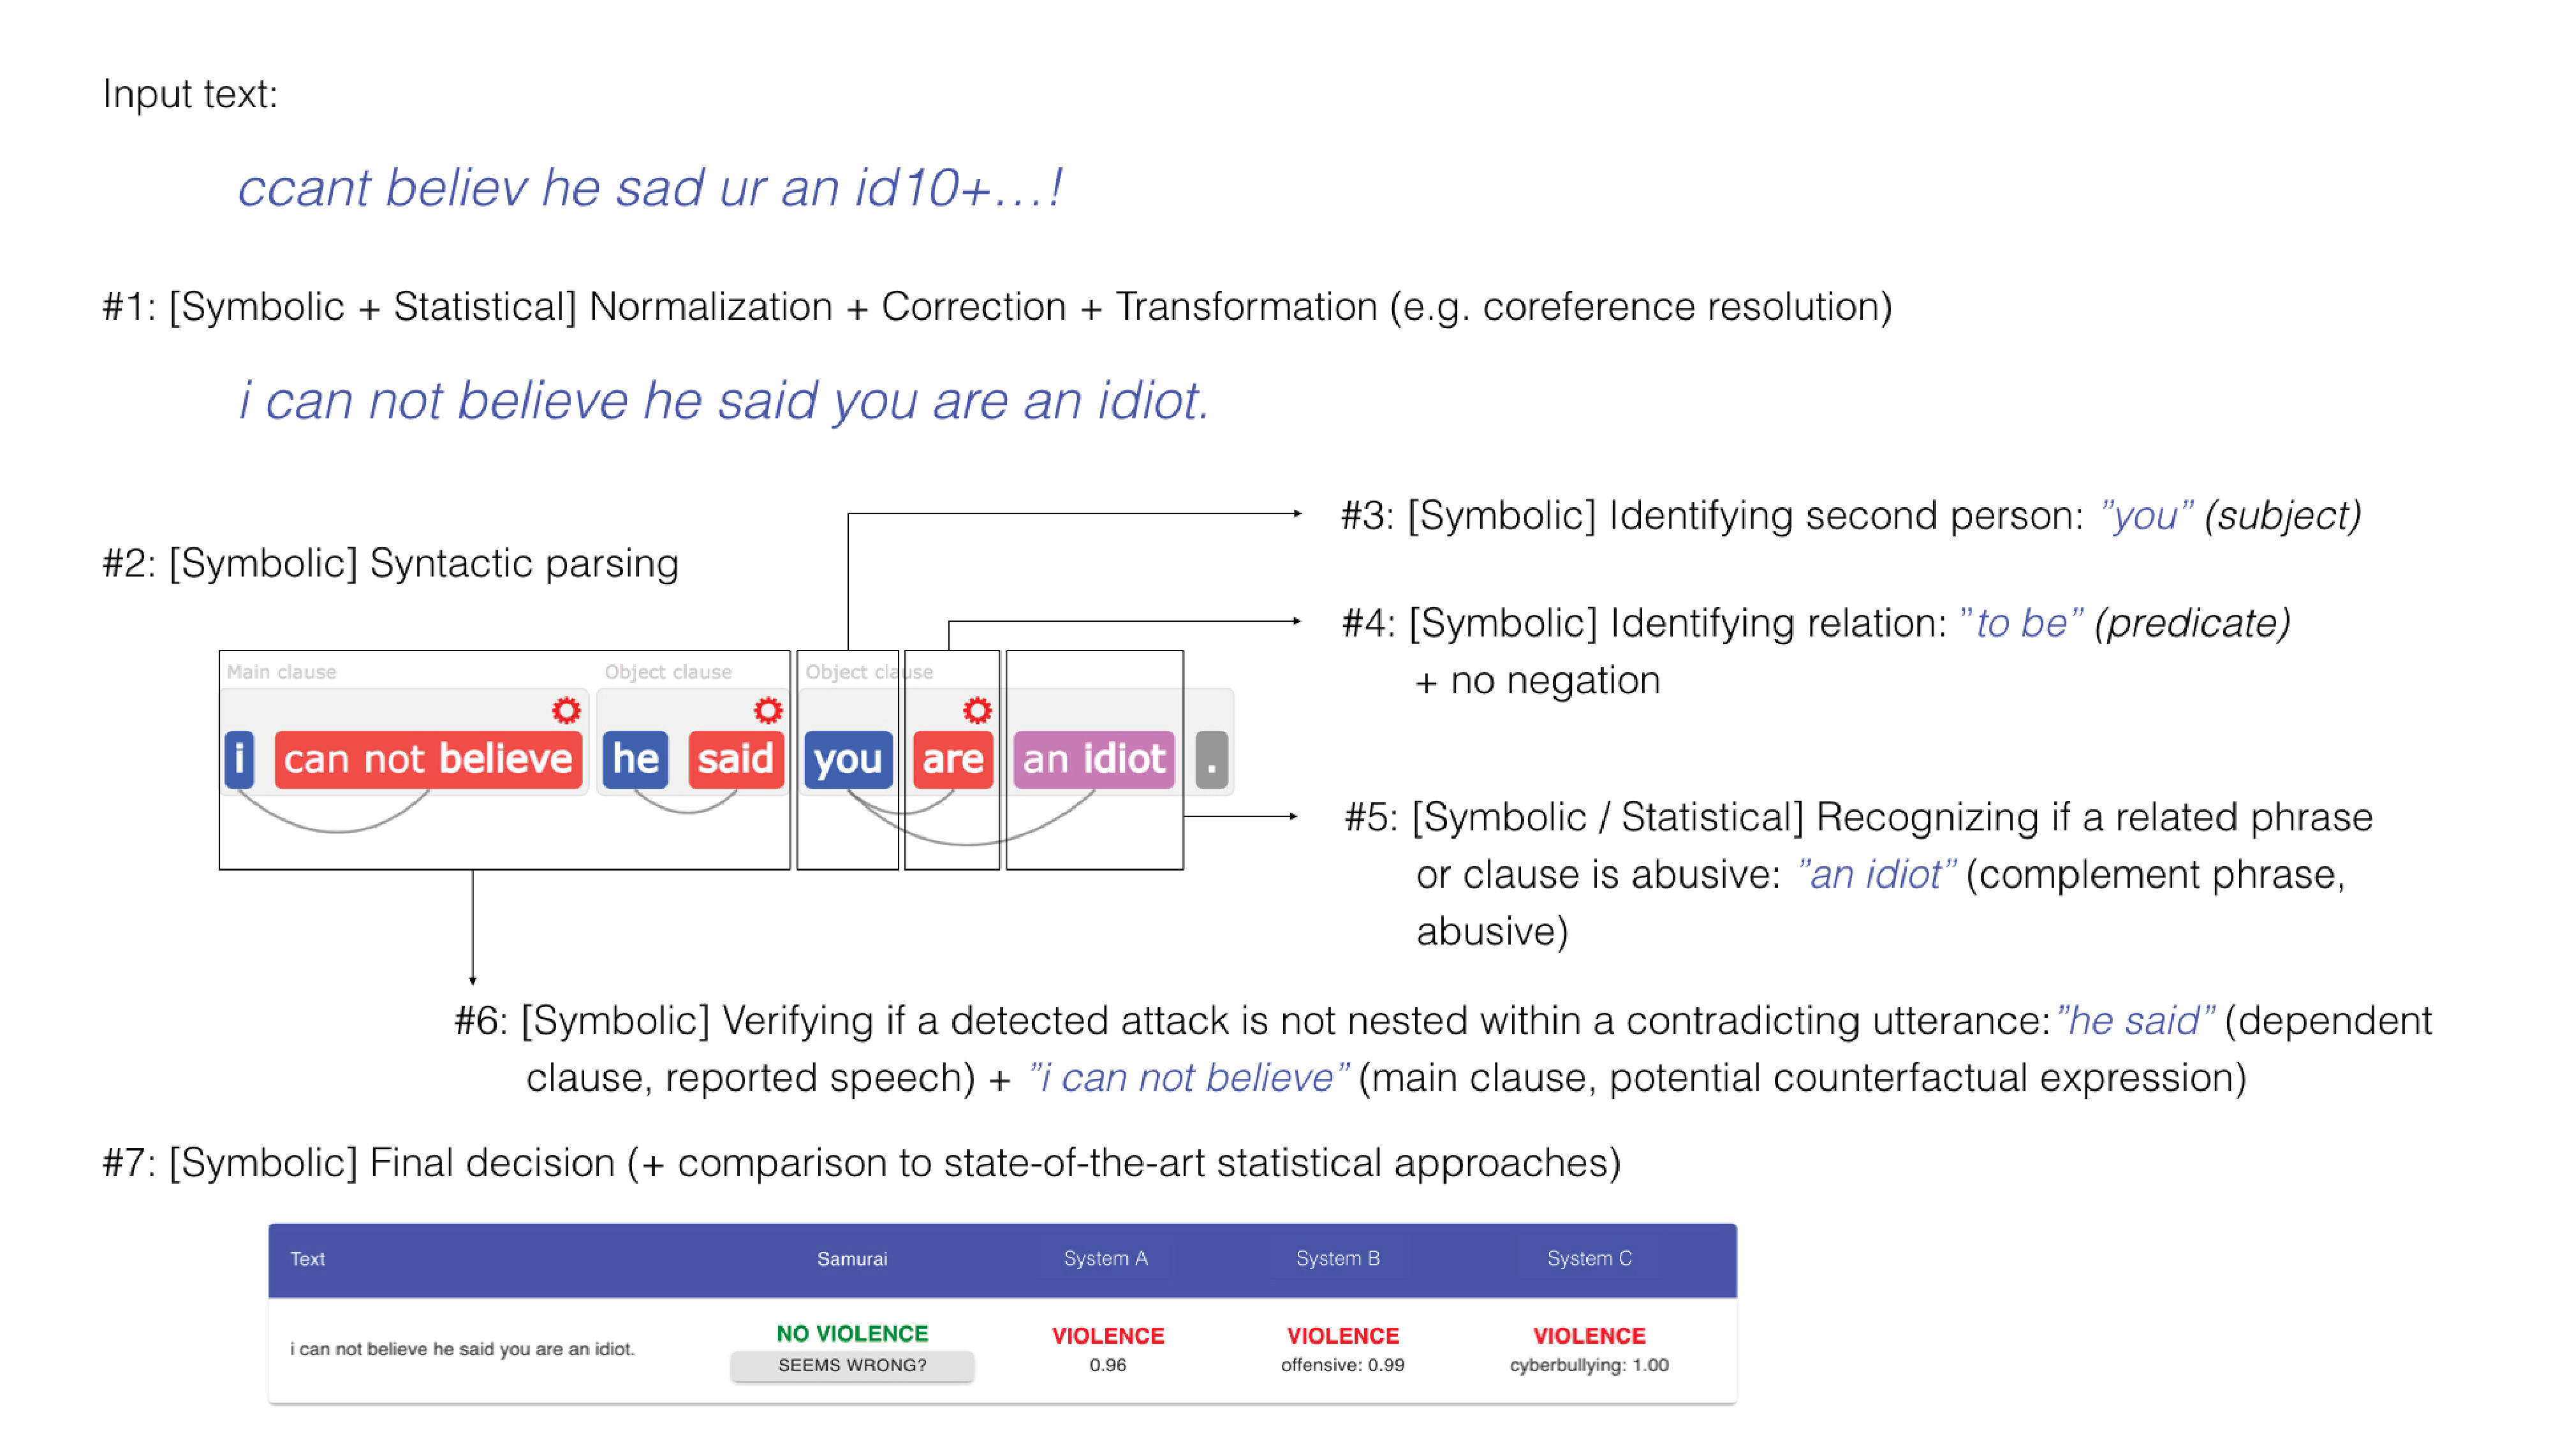
\includegraphics[width=\linewidth]{../images/example.eps}
    \caption{Example of processing of one sentence by the applied Samurai technology.}
    \label{fig:samuraiexample}
\end{figure}

In practice, it means that a whole variety of constructions can be
detected without the need to construct a fixed list of dictionary words
defined \textit{a priori}. Due to utilizing symbolic components that
oversee statistical components, \{\textsf Samurai\} recognizes complex
linguistic phenomena (such as indirect speech, rhetorical figures or
counter-factual expressions) to distinguish personal attacks from normal
communication, greatly reducing the number of false alarms as compared
to others systems used for violence detection. An example of comparison
can be seen in Figure \ref{fig:samuraiexample}, and a full benchmark was
presented in (Ptaszyński, Leliwa, Piech, \& Smywiński-Pohl, 2018).

The detection models utilized in this research were designed to detect
personal attacks targeted against a second person (e.g.~interlocutor,
original author of a post) and a third person/group (e.g., other
participants in the conversation, people not involved in the
conversation, social groups, professional groups), except public figures
(e.g.~politicians, celebrities). With regards to symbolic component of
the system, by ``models'' we mean separate rules (such as, specifying a
candidate for the presence of personal attack, such as the aggressive
word ``idiot,'' which is further disambiguated with a syntactic rule of
citation, e.g., ``{[}he\(\vert\)she\(\vert\)they{]} said {[}SUBJECT{]}
{[}PREDICATE{]}'') or sets of rules, as seen in Figure
\ref{fig:samuraiexample}, e.g.~normalization model contains rules for
transcription normalization, citation detection model contains rules for
citation, etc. With regards to the statistical component, by ``models''
refer to machine learning models trained on large data to classify an
entry into one of the categories (e.g., true personal attack, or false
positive).

Moreover, the symbolic component of the system uses two types of
symbolic rules, namely ``narrow rules'' and ``wide rules.'' The former
have smaller coverage (e.g., are triggered less often), but detect
messages containing personal attacks with high
precision.\footnote{Precision is defined traditionally as the ratio of correctly detected instances among all detected instances.}
The latter, have wider coverage, but their precision is lower. We
decided to set apart the ``narrow'' and ``wide'' subgroups of the
detection models in order to increase the granularity of the analysis.
Firstly, we took only the detection models designed to detect personal
attacks targeted against second person. Secondly, we used these models
on a dataset of 320,000 Reddit comments collected on 2019/05/06.
Thirdly, we randomly picked at most hundred returned results for each
low-level
model\footnote{Low-level models are responsible for detecting low-level categories. Similarly, mid-level models detect mid-level categories, by combining several low-level models, etc.}
(some models are triggered very often while others rarely, so using all
instances would create too much bias). There were 390 low-level models
but many of them returned in less than 100 results. We verified them
manually with the help of expert annotators trained in detection of
personal attacks and selected only those models that achieved at least
90\% of precision. The models with fewer than 100 returned results were
excluded from the selection. After this step, the ``narrow'' subgroup
contained 43 out of 390 low-level models. Finally, we tested all of the
``narrow'' models on a large dataset of 477,851 Reddit comments
collected between 2019/06/01 and 2019/08/31 from two subreddits
(r/MensRights and r/TooAfraidToAsk). Each result of the ``narrow''
models was verified manually by a trained annotator and the ``narrow''
models collectively achieved over 93.3\% of precision. We also tested
the rest of the ``wide'' models on random samples of 100 results for
each model (from the previous dataset of 320,000 Reddit comments) and we
excluded the models that achieved less than 80\% precision. The models
with fewer than 100 results were not excluded from the ``wide'' group.
In this simple setup we detected 24,251 texts containing ``wide''
attacks, where:

\begin{itemize}
\item  5,717 (23.6\%) contained personal attacks against second person detected by the "narrow" models,
\item  8,837 (36.4\%) contained personal attacks against second person detected by "wide" models
% the models other than "narrow",
\item  10,023 (41.3\%) contained personal attacks against third persons / groups.
The sum exceeds 100\% because some of the comments contained personal attacks against both second person and third person / groups. For example, a comment ``Fu$\ast\ast$ you a$\ast\ast$hole, you know that girls from this school are real bit$\ast\ast$es" contains both types of personal attack.
\end{itemize}

\section{Large-scale quantitative analysis of impact of personal attacks on
Reddit user activity}
\label{quantanalysis}

At this point we move on to the presentation of our observational study.
It is crucial to emphasize that due to space limitations some technical
details and methodological decisions have not been fully explained in
the publication, but we did our best to expand on such issues in the
online documentation of the study.

\subsection{Study design and data collection}

The raw datasets used have been obtained by \textsf{Samurai Labs}, who
were able to collect \textsf{Reddit} posts and comments without
\textsf{Reddit} moderation or comment removal. All content was
downloaded from the data stream provided by \url{pushshift.io} which
enabled full data dump from Reddit in real-time. The advantage of using
it was access to unmoderated data. Further, \textsf{Samurai Labs}
deployed their personal attacks recognition algorithms to identify
personal attacks.

Experimental manipulation of the crucial independent variables (personal
attacks of various form) would be unethical and against the goal of
\textsf{Samurai Labs}, which is to detect and \emph{prevent} online
violence, so this is an observational study. While this is a weakness,
our sample was both much larger and much more varied than the usual
WEIRD (western, educated, and from industrialized, rich, and democratic
countries) groups used in psychology (notice, however, that the majority
of Reddit users are males based in the U.S.).\footnote{For instance,
  Wise, Hamman, \& Thorson (2006) examined 59 undergraduates from a
  political science class at a major Midwestern university in the USA,
  Zong, Yang, \& Bao (2019) studied 251 students and faculty members
  from China who are users of WeChat, and Valkenburg, Peter, \& Schouten
  (2006) surveyed 881 young users (10-19yo.) of a Dutch SNS called CU2.}

Practical limitations allowed for data collection for around two
continuous weeks (day 0 \(\pm\) 7 days). First, we randomly selected one
weekend day and one working day. These were June 27, 2020 (Saturday,
\textsf{S}) and July 02, 2020 (Thursday, \textsf{R}). The activity on
those days was used to assign users to groups in the following manner.
We picked one weekend and one non-weekend day to correct for activity
shifts over the weekend (the data indeed revealed slightly higher
activity over the weekends, no other week-day related pattern was
observed). We could not investigate (or correct for) monthly activity
variations, because the access to unmoderated data was limited. For each
of these days, a random sample of 100,000 posts or comments have been
drawn from all content posted on \textsf{Reddit}. Bot removal and
cleanup left us with 92,943 comments or posts by 75,516 users for
\textsf{R} and 89,585 comments by 72,801 users for \textsf{S}. On these
two days respectively, 1359 \textsf{R} users (\(1.79\%\)) received at
least one \textsf{narrow} attack, 35 of them received more than one
(\(0.046\%\)). 302 of \textsf{S} users (\(0.39\%\)) received at least
one \textsf{narrow} attack and 3 of them more than one \textsf{narrow}
on that day (\(0.003\%\)). These numbers are estimates for a single day,
and therefore if the chance of obtaining at least one \textsf{narrow}
attack in a day is \(1.79\%\), assuming the binomial distribution, the
estimated probability of obtaining at least one \textsf{narrow} attack
in a week is 11.9\% in a week and 43\% in a month. We kept the full
\textsf{wide > 1} or \textsf{narrow > 1} classes comprising 340 users,
and included all of them in the Thursday treatment group
(\textsf{Rtreatment}). Other users were randomly sampled from
\textsf{wide > 0} and added to \textsf{Rtreatment}, so that the group
count was 1000. An analogous strategy was followed for \textsf{S}. 1338
users belonged to \textsf{wide > 0}, 27 to \textsf{wide > 1}, 329 to
\textsf{narrow > 0} and 3 to \textsf{narrow > 1}. The total of 344
\textsf{wide > 1} or \textsf{narrow > 1} users was enriched with sampled
\textsf{wide > 0} users to obtain the \textsf{Streatment} group of 1000
users. The preliminary \textsf{Rcontrol}/\textsf{Scontrol} groups of
1500 users each were constructed by sampling 1500 users who posted
comments on the respective days but did not receive any recognized
attacks.

\begin{table}[H]
\footnotesize
\begin{table}[H]
\centering\begingroup\fontsize{9}{11}\selectfont

\begin{tabular}{lr}
\toprule
Group & n\\
\midrule
\cellcolor{gray!6}{Rcontrol} & \cellcolor{gray!6}{875}\\
Rtreatment & 935\\
\cellcolor{gray!6}{Scontrol} & \cellcolor{gray!6}{942}\\
Streatment & 921\\
\bottomrule
\end{tabular}
\endgroup{}
\end{table}
\caption{Study group sizes.}
\label{tab:groups}
\end{table}

For each of these groups new dataset was prepared, containing all posts
or comments made by the users during the period of \(\pm 7\) days from
the selection day (337,015 for \textsf{Rtreatment}, 149,712 for
\textsf{Rcontrol}, 227,980 for \textsf{Streatment} and 196,999 for
\textsf{Scontrol}) and all comments made to their posts or comments
(621,486 for \textsf{Rtreatment}, 170,422 for \textsf{Rcontrol}, 201,614
for \textsf{Streatment} and 204,456 for \textsf{Scontrol}), after
checking for uniqueness these jointly were 951,949 comments for
\textsf{Rtreatment}, 318,542 comments for \textsf{Rcontrol}, 404,535
comments for \textsf{Streatment}, and 380,692 comments for
\textsf{Scontrol}).

\vspace{1mm}

We used the boxplot rule to identify of 534 ``powerusers'' which we
suspected of being bots (even though we already removed users whose
names suggested they were bots) --- all of them were manually checked by
\textsf{Samurai Labs}. Those identified as bots (only 15 of them) or
missing (29 of them) were removed. A few more unusual data points needed
to be removed, because they turned out to be users whose comments
contained large numbers of third-person personal attacks which in fact
supported them. Since we were interested in the impact of personal
attacks directed against a user on the user's activity, such unusual
cases would distort the results. 86 users who did not post anything in
the \textsf{before} period were also removed. In the end, \textsf{R} and
\textsf{S} were aligned, centering around the selection day (day 8) and
the studied group comprised 3673 users (see
\mbox{Table \ref{tab:groups}}).

\subsection{Exploration}

First, we visually explore our dataset by looking at the relationship
between the number of received (narrow) attacks vs.~the activity change
counted as the difference of weekly counts of posts or comments authored
in the second (\textsf{after}) and in the first week (\textsf{before})
(Fig. \ref{fig:highPlots}).\footnote{Visualizations for \textsf{wide}
  and \textsf{wide only} attacks, where a weaker, but still negative
  impact, can be observed can be found in the online documentation.
  There, while the tendency is negative for low numbers of attacks,
  higher numbers mostly third-person personal attacks seem positively
  correlated with activity change. This might suggest that while being
  attacked has negative impact on a user's activity, having your post
  ``supported'' by other users' third-person attacks has a more
  motivating effect. Also keep in mind that the distinction between wide
  and narrow pertains only to the choice of attack recognition algorithm
  and does not directly translate into how offensive an attack was,
  except that \textsf{wide} attacks also include third-person ones. In
  what follows, unless indicated otherwise, by attacks we will mean
  narrow attacks.}

\footnotesize

\normalsize

\begin{figure}

\begin{center}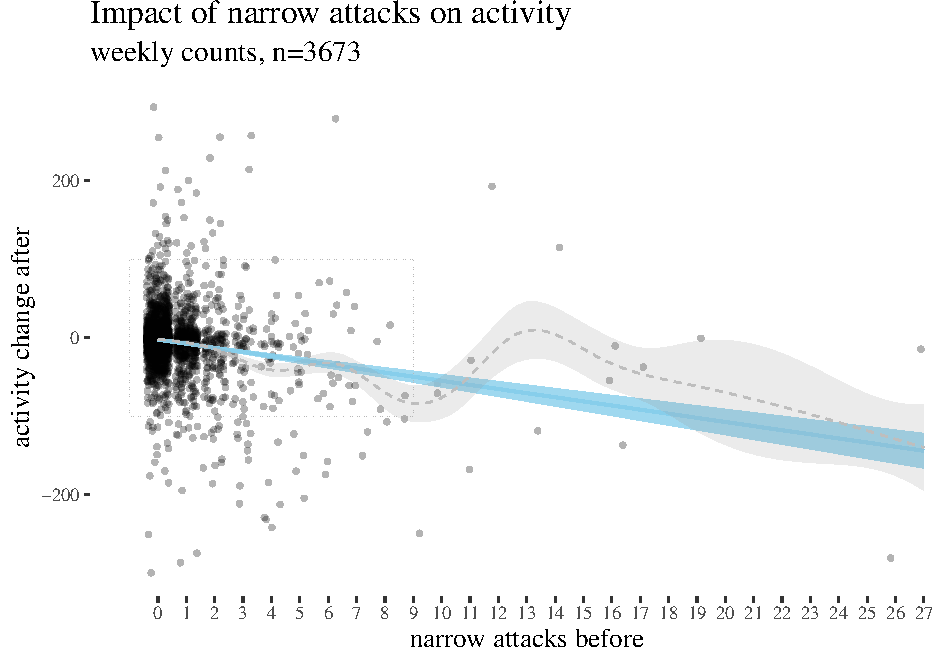
\includegraphics[width=0.85\linewidth]{quittingShortAbridgedRevisions3_files/figure-latex/unnamed-chunk-3-1} \end{center}
\caption{Narrow attacks vs. weekly activity change (jittered), with  linear and gam smoothing.}
\label{fig:highPlots}
\end{figure}

The visualization in Figure \ref{fig:highPlots} should be understood as
follows. Each point is a user. The \(x\)-axis represents a number of
attacks they received in the \textsf{before} period (so that, for
instance, users with 0 wide attacks are the members of the control
group), and the \(y\)-axis represents the difference between their
activity count \textsf{before} and \textsf{after}. We can see that most
of the users received 0 attacks before (these are our control group
members), with the rest of the group receiving 1, 2, 3, etc. attacks in
the \textsf{before} period with decreasing frequency. The blue line
represents linear regression suggesting negative correlation. The gray
line is constructed using generalized additive mode (gam) smoothing,
which is a fairly standard smoothing method for large datasets (it is
more sensitive to local tendencies and yet avoids overfitting). The
parameters of the gam model (including the level of smoothing) are
chosen by their predictive
accuracy.\footnote{See  the documentation of \textsf{gam} of the \textsf{mgcv} packages for details: \url{https://www.rdocumentation.org/packages/mgcv/versions/1.8-33/topics/gam}.}
Shades indicate the 95\% confidence level interval for predictions from
the linear model.

\begin{figure}[H]

\begin{center}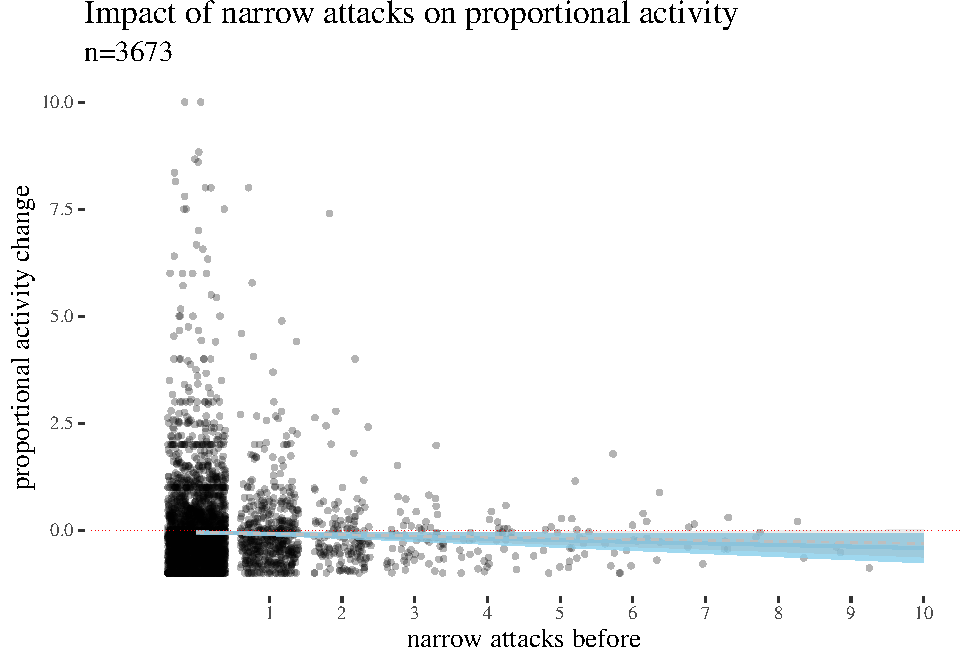
\includegraphics[width=1\linewidth]{quittingShortAbridgedRevisions3_files/figure-latex/unnamed-chunk-7-1} \end{center}
\caption{Impact of attacks  on proportional activity change.}
\label{fig:propActivity}
\end{figure}

Fig. \ref{fig:highPlots} visualizes the activity change in terms of
weekly counts. However, arguably, a change of -20 for a user who posts
500 times a week has different weight than for a user who posts 30
times. For this reason, we also need to look at changes in proportion,
calculated by taking
\(\mathsf{activityScore} = \nicefrac{\mathsf{activityDifference}}{\mathsf{activityBefore}}\).
We zoom in to densely populated areas of the plot for
\textsf{activityScore} as a function of attacks in Figure
\ref{fig:propActivity}. The impact is still negative, more so for
\textsf{narrow} attacks, and less so for other types. For mathematical
reasons the score minimum is -1 (user activity cannot drop more than
100\%).

\subsection{Classical estimation}

Next, we focus on the uncertainties involved. One standard way to
estimate them is to use a one-sample t-tests to estimate the means and
95\% confidence intervals for \textsf{activityDifference} for different
numbers of attacks (this would be equivalent to running a paired t-test
for activity before and activity after). Here is the analysis for narrow
attacks. There were not enough observations for attacks above 8 (3, 2,
and 2 for 9, 10 and 11 attacks, and single observations for a few higher
non-zero counts) for a t-test to be useful, so we run the t-test for up
to 8 attacks. For each type of attack we list 9 options of the number of
attacks and initiate vectors to which we will save the confidence
interval limits (\textsf{low}, \textsf{high}), the estimated mean and
the \textsf{p}-value (Table \ref{tab:testimates}). We use the same
approach to analyze the other types of attacks (Tables
\ref{tab:testimateswide} and
\ref{tab:testimateswideonly}).\footnote{We used t-tests, which one might think assumes normality, to estimate means  for distributions, which in fact  are not normal. However, what t-test assumes is the normality of the sampling distribution, and this condition is much easier to satisfy thanks to the central limit theorem.}

\footnotesize

\normalsize

\footnotesize

\normalsize

\begin{table}[h!]


\begin{table}[H]
\centering\begingroup\fontsize{9}{11}\selectfont

\resizebox{\linewidth}{!}{
\begin{tabular}{lrrrrrrrrr}
\toprule
\cellcolor{gray!6}{attacks} & \cellcolor{gray!6}{0.000} & \cellcolor{gray!6}{1.000} & \cellcolor{gray!6}{2.000} & \cellcolor{gray!6}{3.000} & \cellcolor{gray!6}{4.000} & \cellcolor{gray!6}{5.000} & \cellcolor{gray!6}{6.000} & \cellcolor{gray!6}{7.000} & \cellcolor{gray!6}{8.000}\\
CIlow & -3.154 & -12.658 & -23.390 & -45.991 & -94.861 & -108.030 & -169.527 & -108.555 & -144.273\\
\cellcolor{gray!6}{estimated m} & \cellcolor{gray!6}{-2.140} & \cellcolor{gray!6}{-8.251} & \cellcolor{gray!6}{-12.646} & \cellcolor{gray!6}{-25.607} & \cellcolor{gray!6}{-59.400} & \cellcolor{gray!6}{-60.864} & \cellcolor{gray!6}{-80.882} & \cellcolor{gray!6}{-46.125} & \cellcolor{gray!6}{-46.750}\\
CIhigh & -1.125 & -3.844 & -1.902 & -5.222 & -23.939 & -13.697 & 7.762 & 16.305 & 50.773\\
\cellcolor{gray!6}{p-value} & \cellcolor{gray!6}{0.000} & \cellcolor{gray!6}{0.000} & \cellcolor{gray!6}{0.021} & \cellcolor{gray!6}{0.015} & \cellcolor{gray!6}{0.002} & \cellcolor{gray!6}{0.014} & \cellcolor{gray!6}{0.071} & \cellcolor{gray!6}{0.124} & \cellcolor{gray!6}{0.225}\\
\bottomrule
\end{tabular}}
\endgroup{}
\end{table}

\caption{T-test based estimates for activity change divided by numbers of narrow attacks received.}
\label{tab:testimates}
\end{table}

\begin{table}[h!]


\begin{table}[H]
\centering\begingroup\fontsize{9}{11}\selectfont

\resizebox{\linewidth}{!}{
\begin{tabular}{lrrrrrrrrr}
\toprule
\cellcolor{gray!6}{attacks} & \cellcolor{gray!6}{0.000} & \cellcolor{gray!6}{1.000} & \cellcolor{gray!6}{2.000} & \cellcolor{gray!6}{3.000} & \cellcolor{gray!6}{4.000} & \cellcolor{gray!6}{5.000} & \cellcolor{gray!6}{6.000} & \cellcolor{gray!6}{7.000} & \cellcolor{gray!6}{8.000}\\
CIlow & -3.154 & -12.658 & -23.390 & -45.991 & -94.861 & -108.030 & -169.527 & -108.555 & -144.273\\
\cellcolor{gray!6}{estimated m} & \cellcolor{gray!6}{-2.140} & \cellcolor{gray!6}{-8.251} & \cellcolor{gray!6}{-12.646} & \cellcolor{gray!6}{-25.607} & \cellcolor{gray!6}{-59.400} & \cellcolor{gray!6}{-60.864} & \cellcolor{gray!6}{-80.882} & \cellcolor{gray!6}{-46.125} & \cellcolor{gray!6}{-46.750}\\
CIhigh & -1.125 & -3.844 & -1.902 & -5.222 & -23.939 & -13.697 & 7.762 & 16.305 & 50.773\\
\cellcolor{gray!6}{p-value} & \cellcolor{gray!6}{0.000} & \cellcolor{gray!6}{0.000} & \cellcolor{gray!6}{0.021} & \cellcolor{gray!6}{0.015} & \cellcolor{gray!6}{0.002} & \cellcolor{gray!6}{0.014} & \cellcolor{gray!6}{0.071} & \cellcolor{gray!6}{0.124} & \cellcolor{gray!6}{0.225}\\
\bottomrule
\end{tabular}}
\endgroup{}
\end{table}


\caption{T-test based estimates for activity change divided by numbers of wide attacks received.}
\label{tab:testimateswide}
\end{table}

\begin{table}[h!]

\begin{table}[H]
\centering\begingroup\fontsize{9}{11}\selectfont

\resizebox{\linewidth}{!}{
\begin{tabular}{lrrrrrrrrr}
\toprule
\cellcolor{gray!6}{} & \cellcolor{gray!6}{0.000} & \cellcolor{gray!6}{1.000} & \cellcolor{gray!6}{2.000} & \cellcolor{gray!6}{3.000} & \cellcolor{gray!6}{4.000} & \cellcolor{gray!6}{5.000} & \cellcolor{gray!6}{6.000} & \cellcolor{gray!6}{7.000} & \cellcolor{gray!6}{8.000}\\
lowLo & -3.154 & -12.658 & -23.390 & -45.991 & -94.861 & -108.030 & -169.527 & -108.555 & -144.273\\
\cellcolor{gray!6}{mLo} & \cellcolor{gray!6}{-2.140} & \cellcolor{gray!6}{-8.251} & \cellcolor{gray!6}{-12.646} & \cellcolor{gray!6}{-25.607} & \cellcolor{gray!6}{-59.400} & \cellcolor{gray!6}{-60.864} & \cellcolor{gray!6}{-80.882} & \cellcolor{gray!6}{-46.125} & \cellcolor{gray!6}{-46.750}\\
highLo & -1.125 & -3.844 & -1.902 & -5.222 & -23.939 & -13.697 & 7.762 & 16.305 & 50.773\\
\cellcolor{gray!6}{pLo} & \cellcolor{gray!6}{0.000} & \cellcolor{gray!6}{0.000} & \cellcolor{gray!6}{0.021} & \cellcolor{gray!6}{0.015} & \cellcolor{gray!6}{0.002} & \cellcolor{gray!6}{0.014} & \cellcolor{gray!6}{0.071} & \cellcolor{gray!6}{0.124} & \cellcolor{gray!6}{0.225}\\
\bottomrule
\end{tabular}}
\endgroup{}
\end{table}



\caption{T-test based estimates for activity change divided by numbers of wide only attacks  received.}
\label{tab:testimateswideonly}
\end{table}

\begin{figure}[h!]

\begin{center}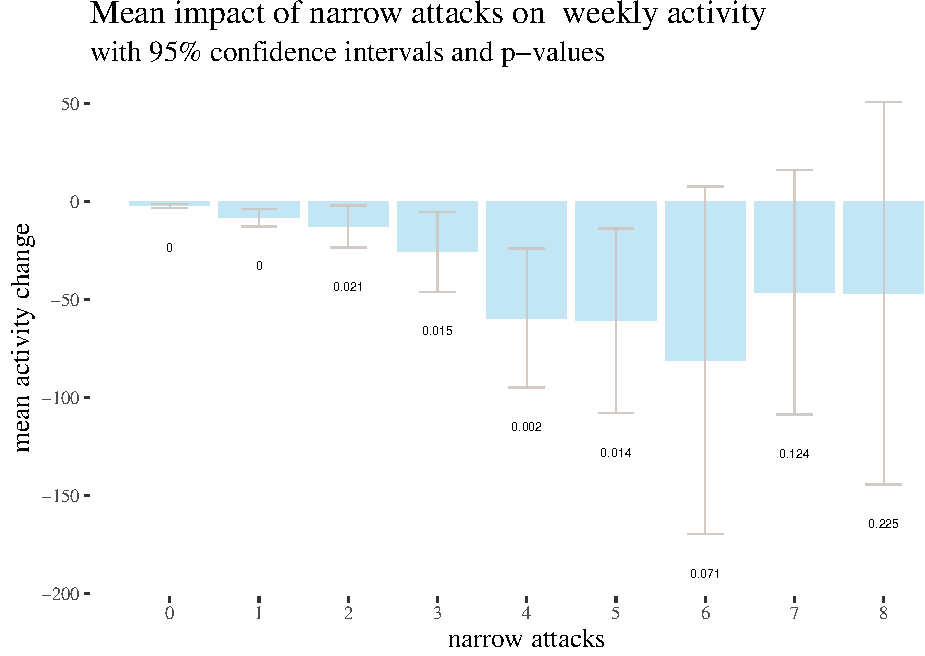
\includegraphics[width=0.95\linewidth]{quittingShortAbridgedRevisions3_files/figure-latex/unnamed-chunk-15-1} \end{center}
\caption{T-test estimation of activity change by narrow attacks received. All available t-tests.}
\label{fig:highbar}
\end{figure}

It might help to visualize this information using barplots. We do so for
narrow attacks (other visualisations are in the online documentation).
The printed values below bars represent \(p\)-values, not the estimated
means (Fig. \ref{fig:highbar}). Note fairly wide confidence intervals
for higher number of attacks. These arise because attacks are quite
rare, so the sample sizes for 5, 6, 7 and 8 narrow attacks are 22, 17, 8
and 4 respectively. This might be also the reason why \(p\)-values are
not too low (although still below the usual significance
thresholds).\footnote{In fact, power analysis shows that if the real activity difference for those groups equals to the mean for \textsf{narrow = 6}, that is, -80, the probabilities that this effect would be discovered by a single sample t-test for 6, 7, and 8 attacks are 0.737, 0.737, 0.309, and so tests for higher numbers of attacks are underpowered.}

\begin{table}[H]
\scalebox{0.82}{

\begin{tabular}{l|r|r|r|r|r}
\hline
  & Df & Sum Sq & Mean Sq & F value & Pr(>F)\\
\hline
narrow & 20 & 785496 & 39274.798 & 25.03076 & 0\\
\hline
residuals & 3652 & 5730212 & 1569.061 &  & \\
\hline
\end{tabular}
}
\caption{ANOVA for activity change vs. narrow \\ attacks received.}
\label{tab:anovanarrow}
\end{table}

We run single t-tests on different groups to estimate different means
and we don't use t-test for hypothesis testing. To alleviate concerns
about multiple testing and increased risk of type I error, we also
performed an ANOVA tests, which strongly suggest non-random correlation
between the numbers of attacks and activity change.

Furthermore, 80 comparison rows in Tukey's Honest Significance Test
(Tukey, 1949) have conservatively adjusted p-value below 0.05. Here we
display only the ANOVA results for narrow attacks, other calculations
are available in the online documentation.

There are, however, some reasons to be concerned with classical methods:

\begin{itemize}
\item
  \(p\)-values and confidence intervals are hard to interpret
  intuitively. For instance, a 95\% confidence interval being \((x,y)\)
  does not mean that the true mean is within \((x,y)\) with probability
  \(0.95\), and the estimated mean being \(z\) with \(p\)-value \(0.01\)
  does not mean that the true population mean is \(z\) with probability
  \(0.99\).
\item
  \(p\)-values and confidence intervals are sensitive to undesirable
  factors, such as stopping intention in experiment design (Kruschke,
  2015).
\item
  Classical hypothesis tests require several assumptions to hold which
  sometimes do not hold in reality, and the choice of significance
  thresholds is arbitrary.
\item
  Crucially, probabilities reported in classical analysis are
  probabilities of the data on the assumption of the null hypothesis
  (e.g., that the true mean is 0), not the posterior probabilities of
  the true parameter values given the data. To obtain these, we used
  Bayesian analysis and studied the impact of skeptical prior
  probabilities on how the data impacts the posterior distribution of
  the parameters at hand.
\end{itemize}

For these reasons, we also analyze the data from a Bayesian perspective.

\subsection{Bayesian estimation}

We used Markov Chain Monte Carlo methods\footnote{We employed the
  \textsf{Bayesian Estimation Supersedes the t-Test} package,
  \url{https://www.rdocumentation.org/packages/BEST/versions/0.5.2}.} to
estimate the posterior probability distribution for mean changes in
activity in different groups.

\begin{figure}[H]

\begin{center}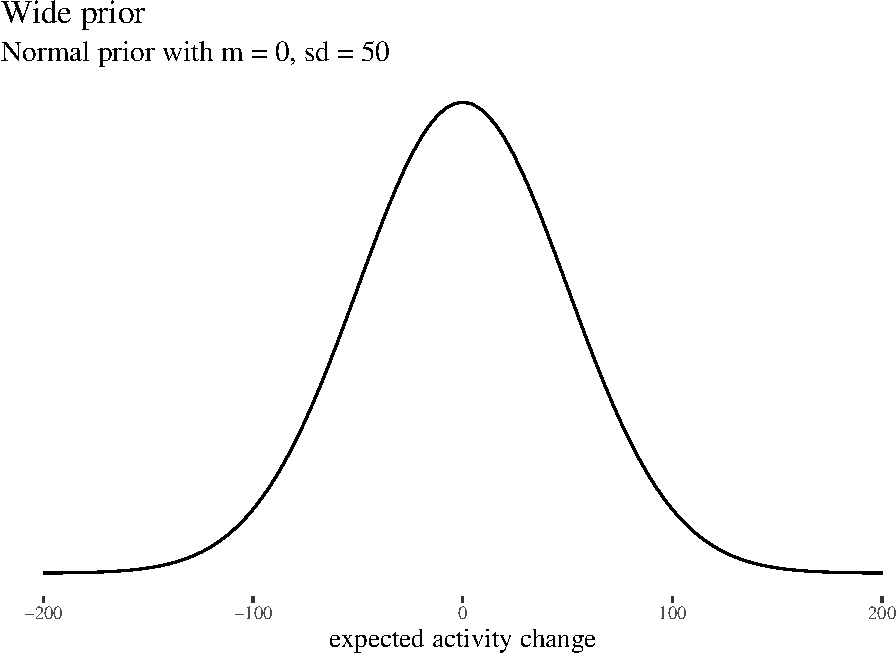
\includegraphics[width=1\linewidth]{quittingShortAbridgedRevisions3_files/figure-latex/unnamed-chunk-20-1} \end{center}
\caption{Wide  skeptical prior for our Bayesian analysis.}
\label{fig:priors}
\end{figure}

We did this for three different fairly skeptical normal prior
distributions (which we call \textsf{wide, informed}, and \textsf{fit}).
In doing so we follow the usual practice of running a Bayesian analysis
with a range of options: the reader is to judge with prior seems most
plausible to them, and then modify their beliefs according to the impact
the data has on their prior convictions. All three distributions are
fairly skeptical because they expect the change to be the same for every
user, and they expect this change to be near 0.\\
Here, due to space limitations, we focus on the wide prior (Fig.
\ref{fig:priors}) , which is normal with \((\mu = 0, \sigma = 50)\).

\noindent  The impact on other priors is studied in the online
documentation, but the results don't differ too
much.\footnote{Their  parameters are respectively $, (\mu = -1.11, \sigma = 44.47)$ and $(\mu = -1.11, \sigma = 7.5)$.   $-1.11$ is the whole sample mean, $44.47$ is the sample standard deviation, and $7.5$ is the standard deviation obtained by  trying to make  theoretical normal distribution similar to the empirical distribution. We did not use  a completely uninformed uniform prior, because it is  not sufficiently skeptical, being more easily impacted by the data, and because it has some undesirable mathematical properties, see \emph{Don’t Use Uniform Priors. They statistically don’t make sense.} at \url{https://towardsdatascience.com/stop-using-uniform-priors-47473bdd0b8a} for an accessible explanation.}

\normalsize

\footnotesize

\normalsize

Here are the results of the Bayesian analysis for 0-9 narrow attacks
(and a simulated prior) for the wide prior and the barplot of the means
of posterior distributions (not the means of the data, but a result of a
compromise between the priors and the data) with highest density
intervals (\ref{fig:bayesian1}).

\begin{figure}[H]

\begin{center}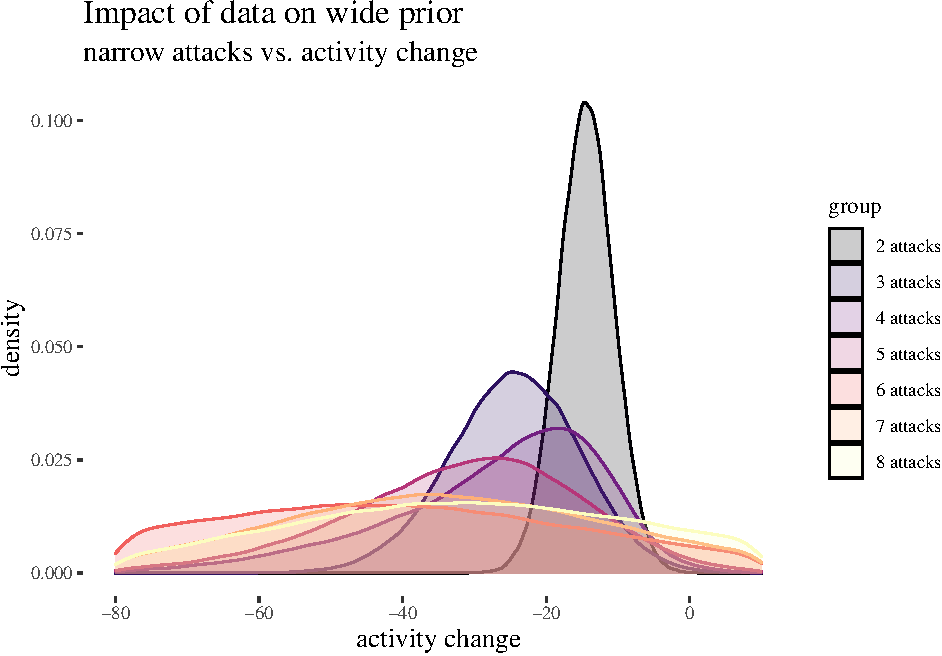
\includegraphics[width=1\linewidth]{quittingShortAbridgedRevisions3_files/figure-latex/unnamed-chunk-25-1} \end{center}
\caption{Posterior distribution for $\geq 2$ attacks and wide priors (lower number of attacks removed, because their high density would adversely affect visibility, see the barplot below for results).}
\label{fig:bayesian1}

\end{figure}

\begin{figure}[H]

\begin{center}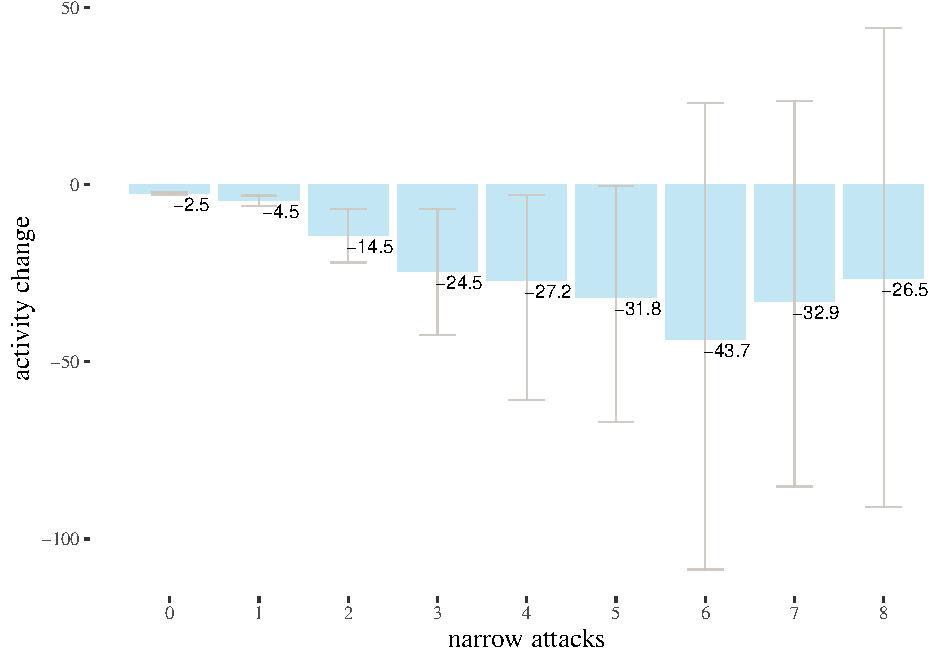
\includegraphics[width=1\linewidth]{quittingShortAbridgedRevisions3_files/figure-latex/unnamed-chunk-26-1} \end{center}
\caption{Posterior means and HDI limits for the wide prior.}
\end{figure}

As the number of attacks grows, no matter which prior we start with, the
posterior means move left (which agrees with the results we obtained
with other methods) and the density plots become wider.

\normalsize

\subsection{Model-theoretic analysis}

\normalsize

We analyzed the correlation between attacks received and activity change
using classical and bayesian methods. However, there is a number of
predictors we have not yet used. The impact of some of them, such as the
number of attacks on \emph{posts} written by an author, could provide
further insight. More importantly, some of them might be confounding
variables. Crucially, since previous activity seems to be a good
predictor of future activity and since high number of attacks received
in the \textsf{before} period correlates with high activity before, one
might be concerned that whatever explaining the value of high attacks
before does in our analysis should actually be attributed simply to
activity.

To reach some clarity on such issues, we perform a regression analysis
to see how the predictors in best fit models interact, and to use the
model parameters to get some comparison of the impact they have. We
build a number of potentially viable generalized linear regression
models meant to predict \textsf{activityAfter} based on a selection of
other variables, pick the best one(s) and analyze what they reveal about
the predictors involved.

\footnotesize

\normalsize

\begin{figure}[H]

\begin{center}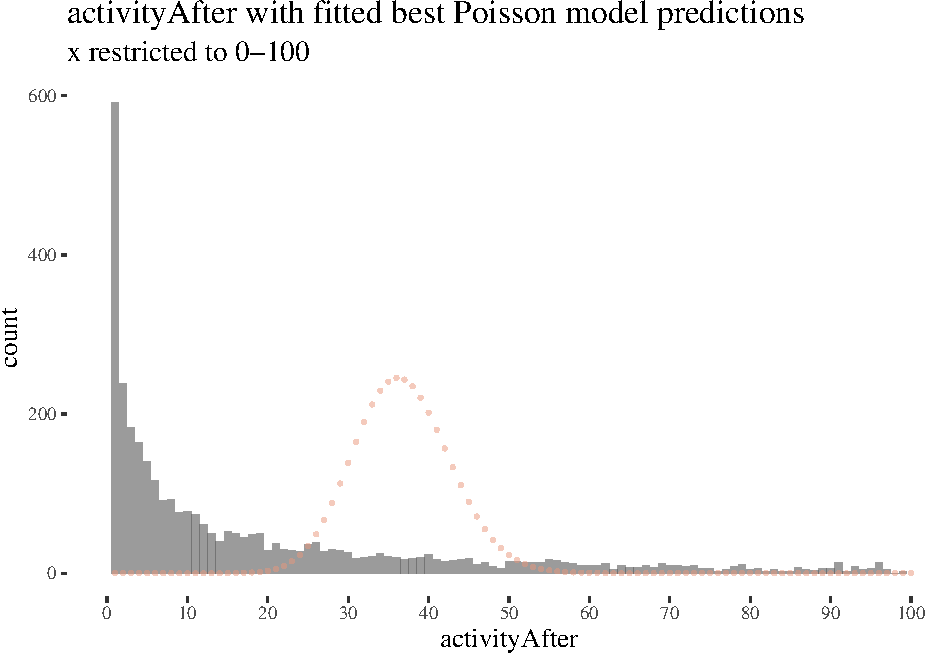
\includegraphics[width=1\linewidth]{quittingShortAbridgedRevisions3_files/figure-latex/unnamed-chunk-32-1} \end{center}
\caption{Poor performance of best-fitting Poisson distribution.}
\label{fig:poissBad}
\end{figure}

Our first challenge was finding the right distribution for the outcome
variable. One potential candidate was the Poisson distribution. We
identified the Poisson distribution that best fits the data, used its
\(\lambda\) parameter (\(\approx 35.69\)) to perform a goodness-of-fit
test (with \(df=273\), \(\chi^2 \approx \infty\) and
\(P(>\chi^2)\approx 0\)), and compare visually the predicted values with
the actual ones (Fig: \ref{fig:poissBad}).

There were at least two problems: zero-inflation and overspread. The
former means that the model predicts much fewer zeros than there really
are in the data, and the latter means that the model predicts fewer
higher values than there are in the data. The best fitting \(\lambda\)
was fairly high and moved the highest values of Poisson too far to the
right compared to where they were expected. Over-dispersion could be
handled by moving to a quasi-Poisson distribution, but this would not
help us much with the zero counts.

\footnotesize

\normalsize

\begin{figure}[H]

\begin{center}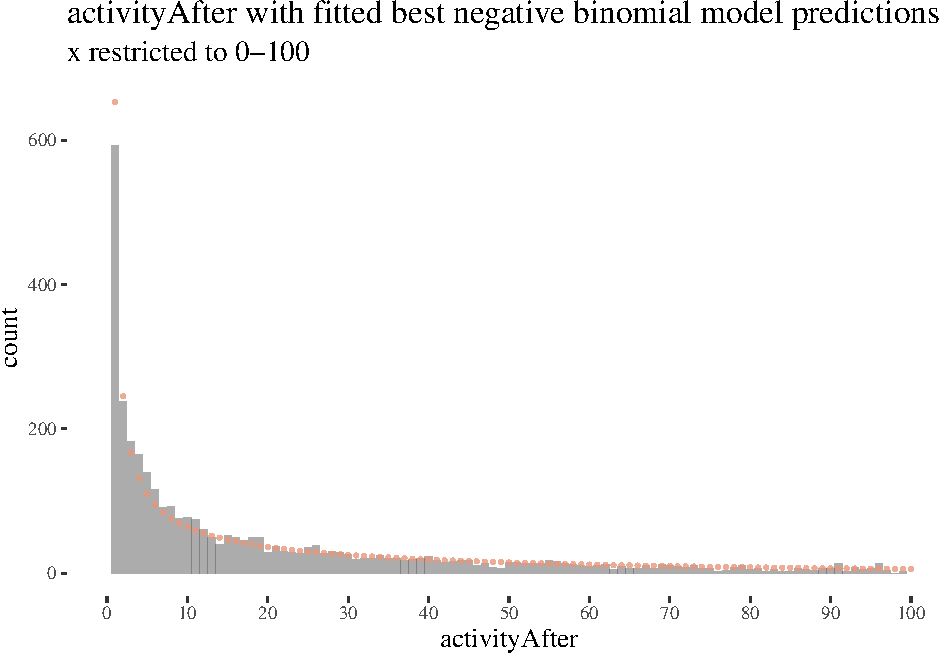
\includegraphics[width=1\linewidth]{quittingShortAbridgedRevisions3_files/figure-latex/unnamed-chunk-35-1} \end{center}
\caption{Somewhat better performance of best-fitting negative binomial distribution.}
\label{fig:nbinperf}
\end{figure}

Another candidate distribution we considered was negative binomial.
There still were problems with zeros although in the opposite direction
though), the goodness-of-fit test resulted in \(\chi^2 \approx 647\) and
\(P(>\chi^s)\approx 0\), but the right side of the Figure
\ref{fig:nbinperf} looks better. This suggested that improvements were
still needed.

There are two well-known strategies to develop distributions for data
with high zero counts: zero-inflated and hurdle
models.\footnote{In a zero-inflated Poisson (ZIP) model (Lambert 1992) a distinction is made between   the structural zeros for which the output value  will always be 0, and the rest, sometimes giving random zeros. A  ZIP model is comprised of two components:

\begin{itemize}
\item  A model for the binary event of membership in the class where 0 is necessary. Typically, this is logistic regression. 

\item  A Poisson (or negative binomial) model for the remaining observed count, potentially including some zeros as well. Typically a log link is used to predict the mean.
\end{itemize}


In hurdle models (proposed initially by Cragg (1971) and developed further by Mullahy (1986)) the idea  is that there may be some special  “hurdle” required to reach a positive count. The model  uses:

\begin{itemize}
\item A logistic regression  submodel to distinguish counts of zero from larger counts, and
\item  Truncated Poisson (or negative binomial) regression for the positive counts  excluding the zero counts.
\end{itemize}} We studied these variants. The first observation was that
even zero-inflation or hurdling do not improve the Poisson distribution
much. The second was that once we use negative binomial distribution,
improvement is obtained, but it does not seem to make much of a
difference whether we use zero-inflation or hurdling. We investigated
this further. One method of comparing such models is the Vuong test
which produced \(z\)-statistic (\(2.08\) with \(p\approx 0.018\))
suggesting the zero-inflated negative binomial model is better than
hurdle negative binomial. However, the differences in log-likelihood
(14459 vs.~14527) and AIC (28945 vs.~29081) were not large.

\footnotesize

\normalsize

\footnotesize

\normalsize

\footnotesize

\normalsize

We build zero-inflated negative binomial and hurdle negative binomial
models, one with all variables, and one based on previous activity only.
If we can get equally good predictions using previous activity only and
ignoring information about attacks, this would suggest no impact of the
other variables.

\footnotesize

\normalsize

Zero-inflated models under-predict low non-zero counts, while hurdle
models are a bit better in this respect, so we focused on them (see the
rootograms available in the online documentation for details). We then
compared the hurdle models using likelihood ratio test, which results in
\(\chi^2 \approx 20.28\), with \(P(>\chi^2)\approx 0.009\). Wald's test
is somewhat similar (ableit more generally applicable). It also
indicates that the additional variables are significant
(\(\chi^2 \approx 24.71\) with \(P(>\chi^2)\approx 0.0017\)), which
suggests that variables other than previous activity are also
significant. Finally, Akaike Information Criterion (Akaike, 1974)
provides an estimator of out-of-sample prediction error and penalizes
more complex models. As long as we evaluate models with respect to the
same data, the ones with lower Akaike score should be chosen. Even with
penalty for the additional variables, the full model receives better
score (although the difference is not very large, 29,081 vs.~29,085).

Finally, we can inspect our best fitting HNB model (Tables
\ref{tab:fhnb_estimates1} and \ref{tab:fhnb_estimates2}) and interpret
the result. The output is split into two submodels: one for predicting
zeros, one for the counts. It could be suggested to ignore those
variables whose coefficients are not statistically significant, but
given the already discussed reasons to include these variables, we are
not going to do this (in fact, attaching too much value to statistical
significance thresholds can be pernicious, and also misleading if the
predictors are correlated, as attacks on posts and attacks on comments
may well be). Moreover, the results of step-wise elimination from the
full model are sensitive to the ordering in which we consider variables,
and there is no principled reason to prefer any of the orderings.
Instead, interpreting \(p\)-values we apply the following advice: the
closer it is to 1, the more skeptical we should be about the judgment
the model makes about its role.

\begin{table}[H]
\scalebox{0.75}{
\begin{tabular}{@{\extracolsep{5pt}}lc}
\\[-1.8ex]\hline
\hline \\[-1.8ex]
& \multicolumn{1}{c}{\textit{Dependent variable:}} \\
\cline{2-2}
\\[-1.8ex] & activityAfter \\
\hline \\[-1.8ex]
sumLowOnlyBefore & $-$0.009 \\
& (0.53) \\
& \\
sumHighBefore & $-$0.008 \\
& (0.7) \\
& \\
sumPlBefore & 0.024 \\
& (0.21) \\
& \\
sumPhBefore & $-$0.147 \\
& (0.07) \\
& \\
activityBefore & 0.015$^{***}$ \\
& (2e-16) \\
& \\
Constant & 2.534$^{***}$ \\
& (2e-16) \\
& \\
\hline
\hline \\[-1.8ex]
\textit{Note:} & \multicolumn{1}{r}{$^{*}$p$<$0.1; $^{**}$p$<$0.05; $^{***}$p$<$0.01} \\
\end{tabular}
}
\caption{Estimated parameters of the count part of the  hurdle negative binomial model.}
\label{tab:fhnb_estimates1}
\end{table}

\begin{table}[H]
\scalebox{0.75}{
\begin{tabular}{@{\extracolsep{5pt}}lc}
\\[-1.8ex]\hline
\hline \\[-1.8ex]
& \multicolumn{1}{c}{\textit{Dependent variable:}} \\
\cline{2-2}
\\[-1.8ex] & activityAfter \\
\hline \\[-1.8ex]
sumLowOnlyBefore & $-$0.009 \\
& (0.53) \\
& \\
sumHighBefore & $-$0.008 \\
& (0.7) \\
& \\
sumPlBefore & 0.024 \\
& (0.21) \\
& \\
sumPhBefore & $-$0.147 \\
& (0.07) \\
& \\
activityBefore & 0.015$^{***}$ \\
& (2e-16) \\
& \\
Constant & 2.534$^{***}$ \\
& (2e-16) \\
& \\
\hline
\hline \\[-1.8ex]
\textit{Note:} & \multicolumn{1}{r}{$^{*}$p$<$0.1; $^{**}$p$<$0.05; $^{***}$p$<$0.01} \\
\end{tabular}}
\caption{Estimated parameters of the count part of the  hurdle negative binomial model.}
\label{tab:fhnb_estimates2}
\end{table}

\normalsize

\begin{table}[H]

\begin{table}[H]
\centering\begingroup\fontsize{9}{11}\selectfont

\begin{tabular}{lr}
\toprule
  & Odds ratios\\
\midrule
\cellcolor{gray!6}{count\_(Intercept)} & \cellcolor{gray!6}{12.606}\\
count\_sumLowOnlyBefore & 0.991\\
\cellcolor{gray!6}{count\_sumHighBefore} & \cellcolor{gray!6}{0.992}\\
count\_sumPlBefore & 1.015\\
\cellcolor{gray!6}{count\_sumPhBefore} & \cellcolor{gray!6}{0.870}\\
\addlinespace
count\_activityBefore & 1.015\\
\cellcolor{gray!6}{zero\_(Intercept)} & \cellcolor{gray!6}{1.634}\\
zero\_sumLowOnlyBefore & 0.990\\
\cellcolor{gray!6}{zero\_sumHighBefore} & \cellcolor{gray!6}{0.894}\\
zero\_sumPlBefore & 0.901\\
\addlinespace
\cellcolor{gray!6}{zero\_sumPhBefore} & \cellcolor{gray!6}{1.156}\\
zero\_activityBefore & 1.084\\
\bottomrule
\end{tabular}
\endgroup{}
\end{table}
\caption{Exponentiated coefficient of the full hurdle negative binomial model (rounded).}
\label{tab:exphnb}
\end{table}

The coefficeints are somewhat difficult to interpret because the models
use log link function. Therefore we first exponentiate them to obtain
odds ratios (Table \ref{tab:exphnb}). Let's interpret the intercepts of
the count submodel. The baseline number of posts for those who are not
in the zero class is 12.6. The coefficients indicate that the
multiplicative contribution of each unit change.

We visualise the effects of selected variables by plotting what activity
levels the model predicts for their different values (we focus on 0-40,
as the top of this range is already an extrapolation), while keeping
other variables fixed at their mean values (Figure \ref{fig:effects}).

\footnotesize

\normalsize

To make sure our choice to use the hurdle model was not crucial for
these results, we also provide effect plots for the full zero-inflated
model.

\begin{figure}
\centering

\begin{center}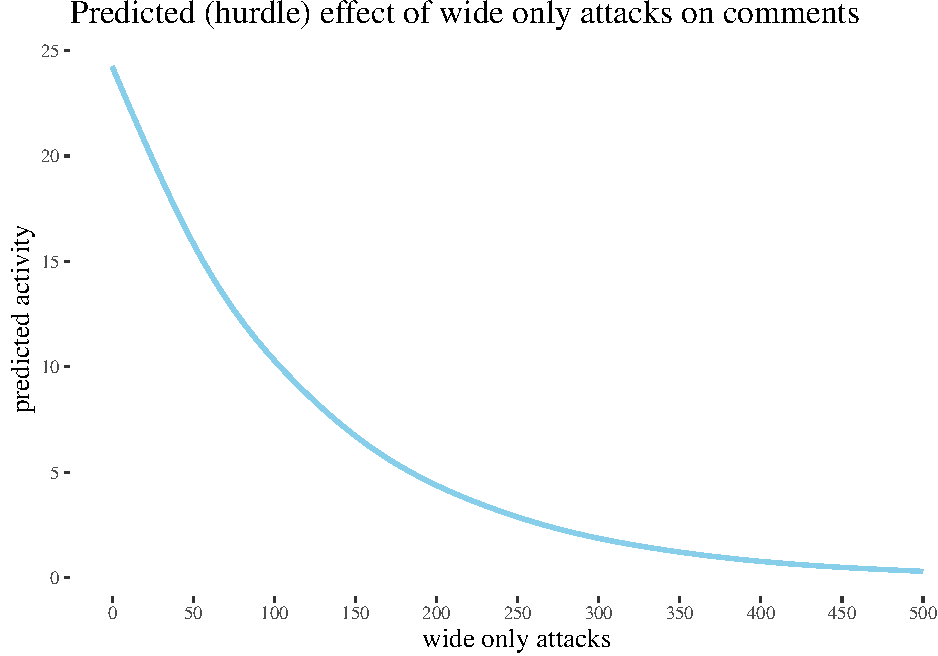
\includegraphics[width=0.85\linewidth]{quittingShortAbridgedRevisions3_files/figure-latex/unnamed-chunk-47-1} \end{center}
\end{figure}

\begin{figure}
\centering

\begin{center}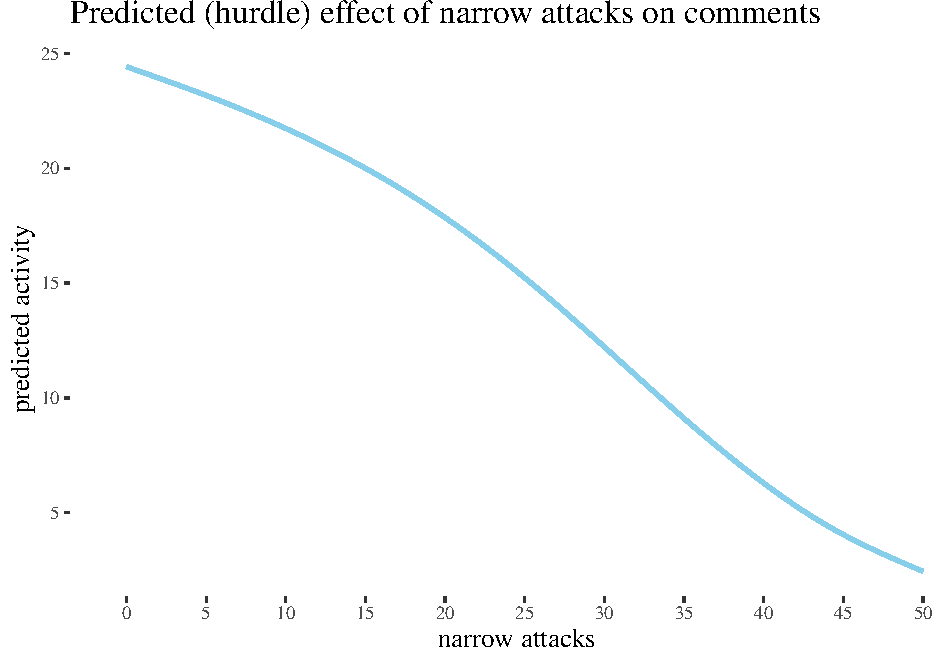
\includegraphics[width=0.85\linewidth]{quittingShortAbridgedRevisions3_files/figure-latex/unnamed-chunk-48-1} \end{center}
\end{figure}

\begin{figure}
\centering

\begin{center}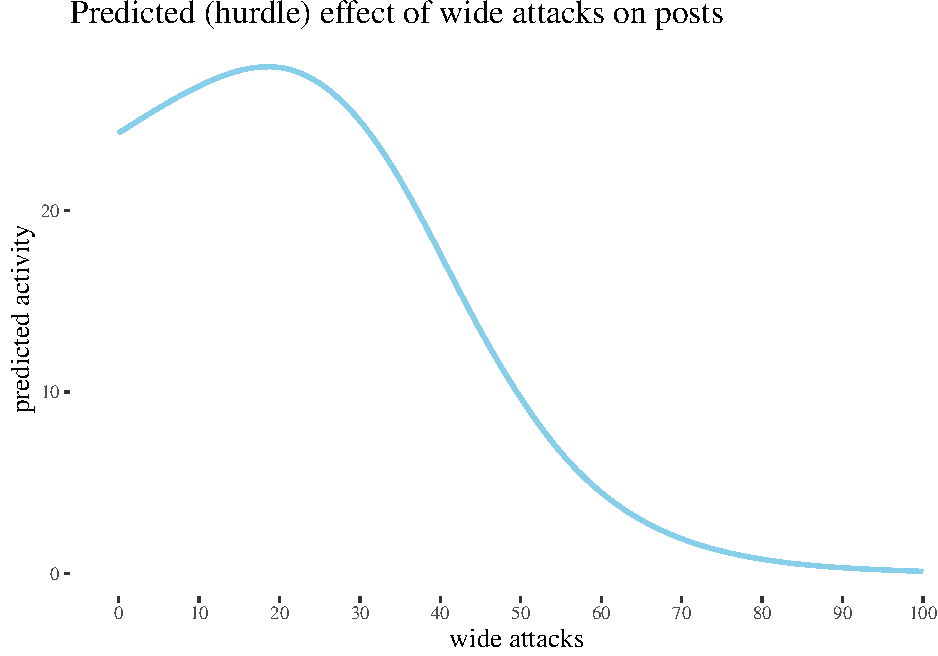
\includegraphics[width=0.85\linewidth]{quittingShortAbridgedRevisions3_files/figure-latex/unnamed-chunk-49-1} \end{center}
\end{figure}

\begin{figure}
\centering

\begin{center}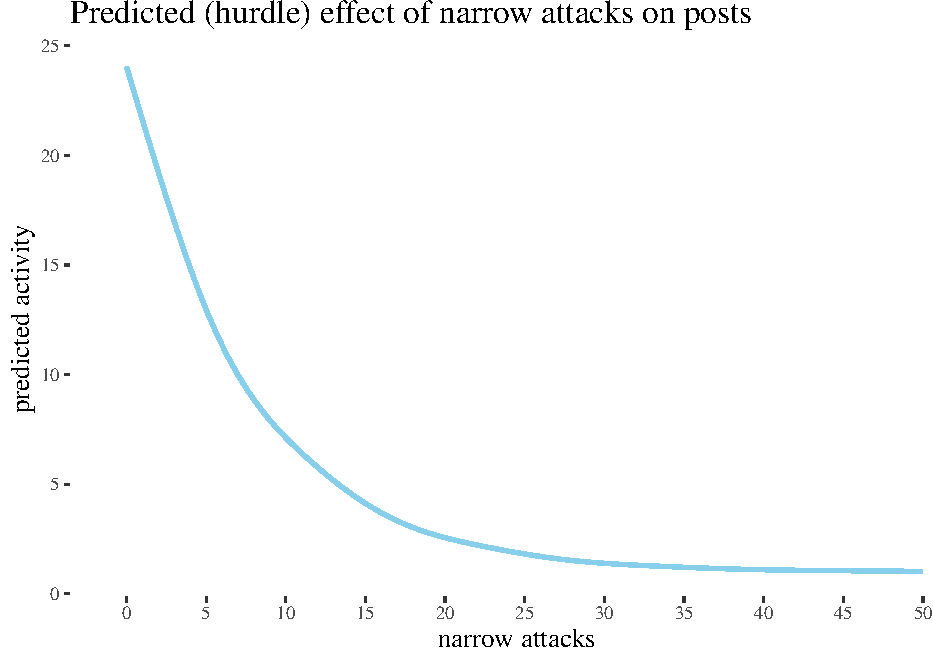
\includegraphics[width=0.85\linewidth]{quittingShortAbridgedRevisions3_files/figure-latex/unnamed-chunk-50-1} \end{center}
\end{figure}

\begin{figure}

\centering

\begin{center}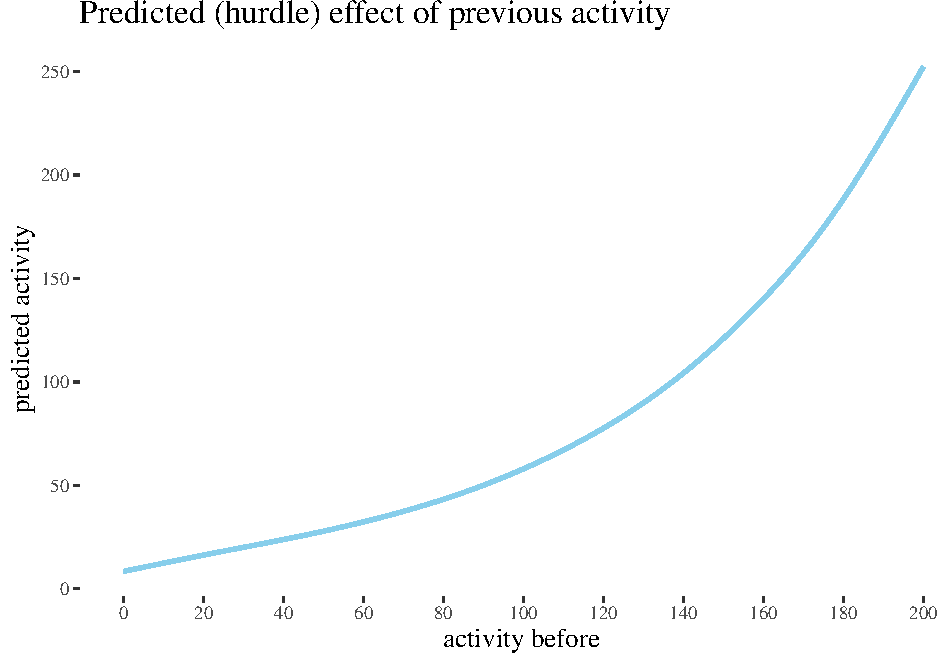
\includegraphics[width=0.85\linewidth]{quittingShortAbridgedRevisions3_files/figure-latex/unnamed-chunk-51-1} \end{center}

\caption{Predicted effects of selected variables on activity with other variables fixed at their mean values, hurdle model.}
\label{fig:effects}
\end{figure}

\footnotesize

\normalsize

\begin{figure}
\centering


\begin{center}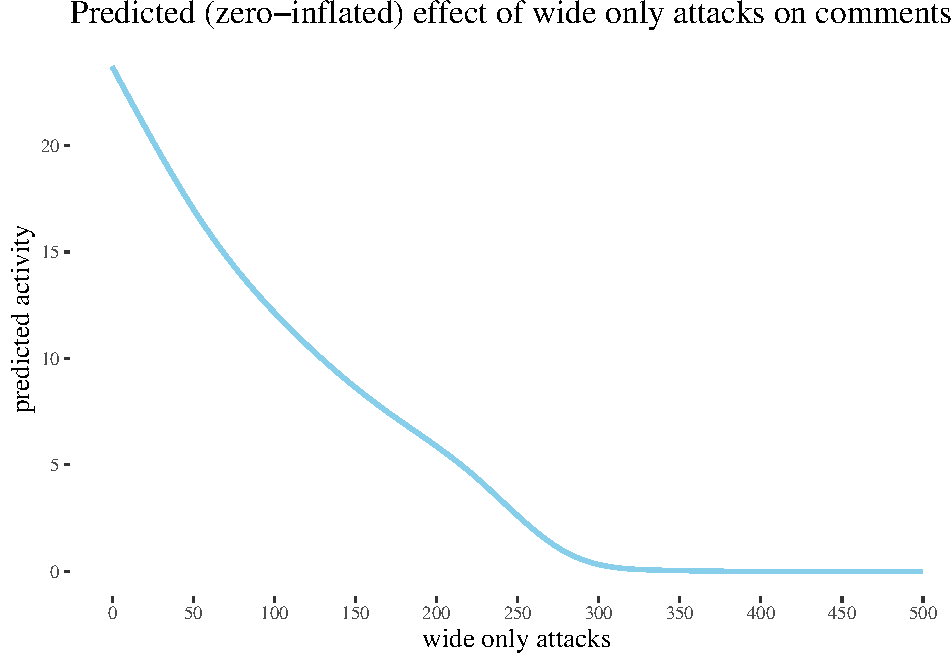
\includegraphics[width=0.85\linewidth]{quittingShortAbridgedRevisions3_files/figure-latex/unnamed-chunk-53-1} \end{center}
\end{figure}

\begin{figure}

\begin{center}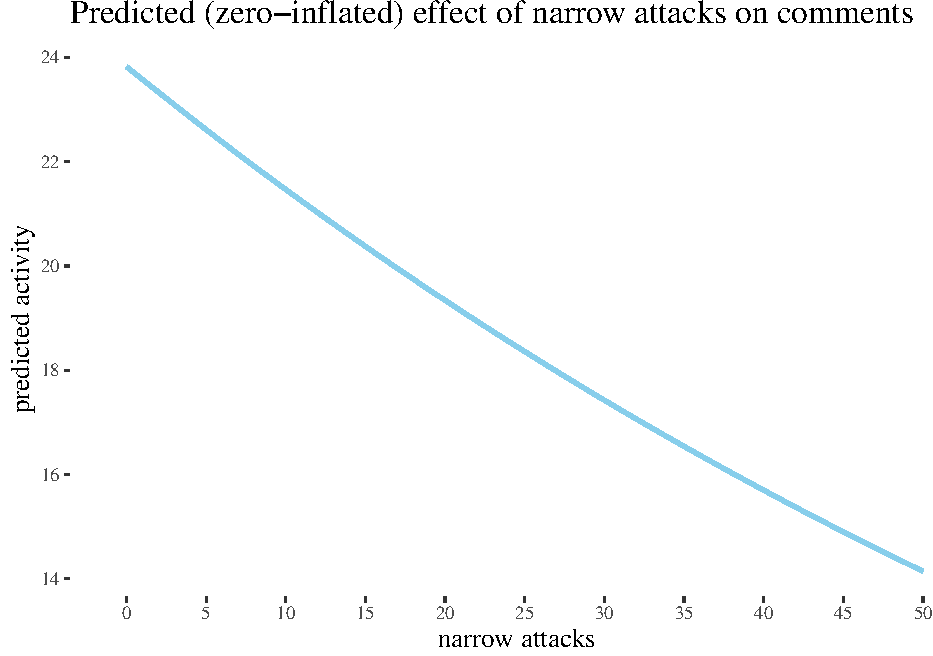
\includegraphics[width=0.85\linewidth]{quittingShortAbridgedRevisions3_files/figure-latex/unnamed-chunk-54-1} \end{center}
\end{figure}

\begin{figure}

\begin{center}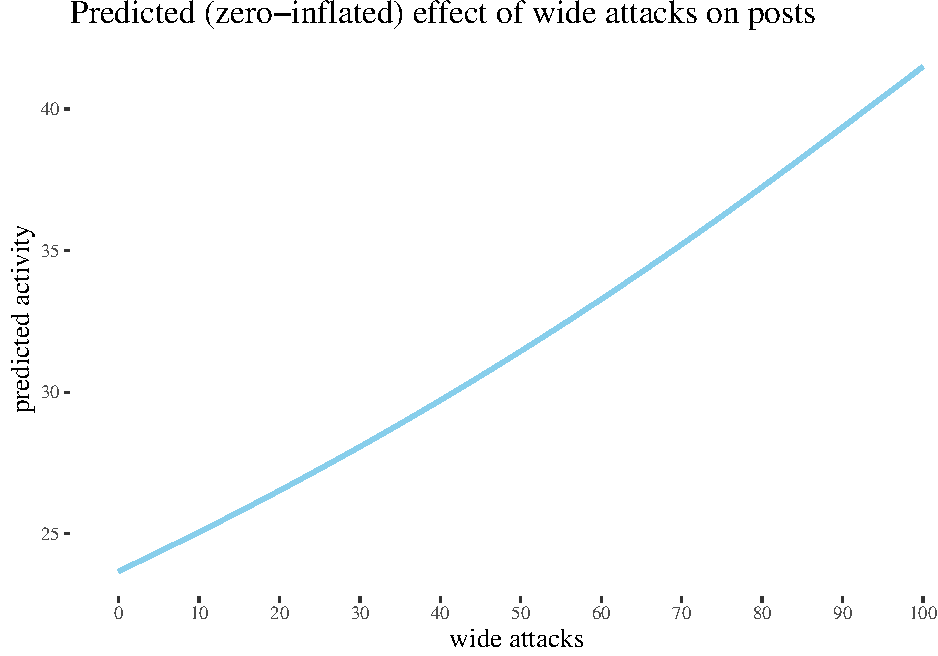
\includegraphics[width=0.85\linewidth]{quittingShortAbridgedRevisions3_files/figure-latex/unnamed-chunk-55-1} \end{center}
\end{figure}

\begin{figure}

\begin{center}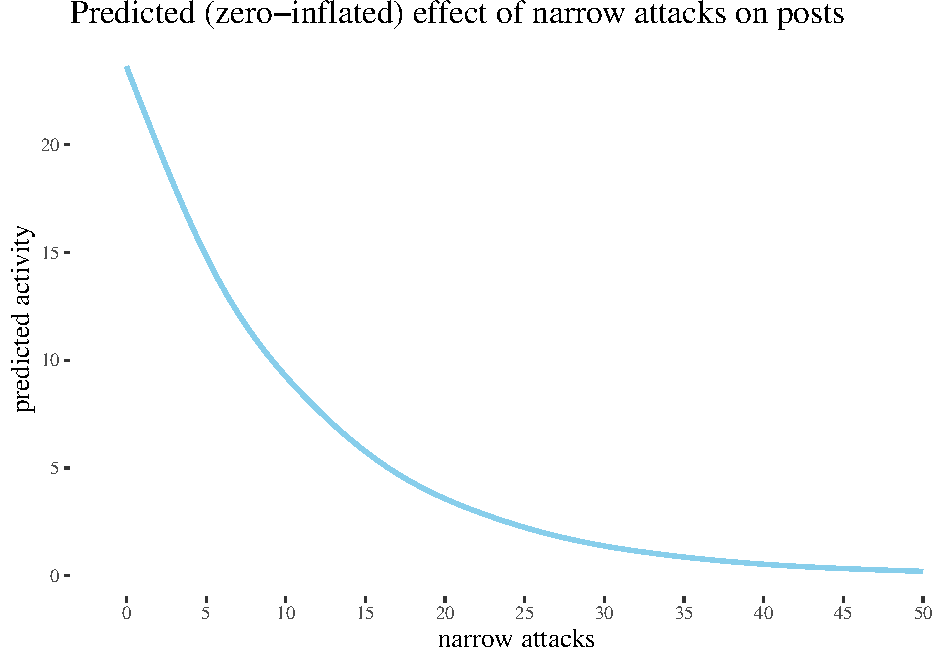
\includegraphics[width=0.85\linewidth]{quittingShortAbridgedRevisions3_files/figure-latex/unnamed-chunk-56-1} \end{center}
\end{figure}

\begin{figure}

\begin{center}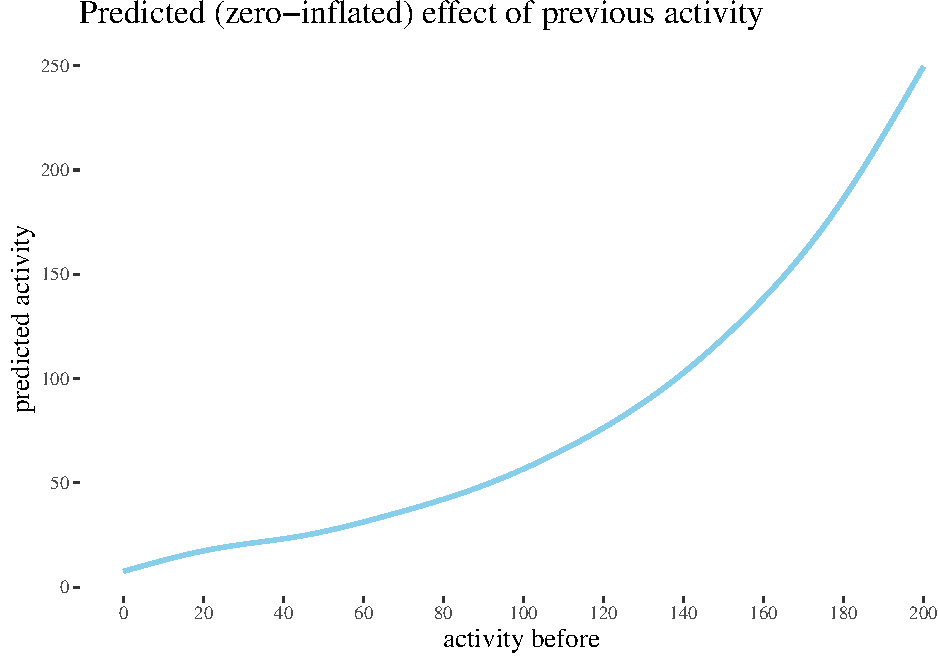
\includegraphics[width=0.85\linewidth]{quittingShortAbridgedRevisions3_files/figure-latex/unnamed-chunk-57-1} \end{center}
\caption{Predicted effects of selected variables on activity with other variables fixed at their mean values, zero-inflated model.}
\label{fig:effects2}
\end{figure}

The predictions are similar, except for the predicted results of wide
only attacks on posts. This perhaps can be explained by observing that
such cases of personal attacks sometimes represent situations in which
the users actually agree with the original post (see our remark in the
beginning of the section about data gathering and selection), and in
some cases the attacks are critical of the author, so there is much more
variation in this group and precise modeling is
harder.\footnote{It should be kept in mind that  the model is built on up to 27 attacks in the \textsf{before} period, with really low number of attacks above 8, so the prediction here is an extrapolation, not an interpolation. Further studies for longer periods are needed to get a more reliable estimate allowing for interpolation in this respect.}
\footnote{One might have reasoned about our previous analyses as follows:  attacks in the before period correlate with activity before, and it is activity before that is the real predictor of activity after. This could be supported by observing that the $p$-value for the hurdle model is really low for activity before.  Pearson correlation coefficient for narrow attacks before and activity before is $r(3671)\approx$ 0.437 and   $r(3671)\approx$ 
0.332 for activity after. However, activity before is a much better correlate of activity after, $r(3671)\approx$ 
0.845 --- all correlations with $p$-value $<2.2e-16$, and regression analysis (inspect the effect plots) indicates that activity before and high attacks before actually go in the opposite directions.}

Another way to use this information is to inspect the table of activity
counts that the model expects based on the number of personal attacks on
a post received in the before period, assuming all the other input
variables are kept at their mean values:

\begin{table}[H]
\begin{table}[H]
\centering\begingroup\fontsize{9}{11}\selectfont

\resizebox{\linewidth}{!}{
\begin{tabular}{lrrrrrrrrrrrrrrrrrrrr}
\toprule
\cellcolor{gray!6}{attacks} & \cellcolor{gray!6}{0} & \cellcolor{gray!6}{1} & \cellcolor{gray!6}{2} & \cellcolor{gray!6}{3} & \cellcolor{gray!6}{4} & \cellcolor{gray!6}{5} & \cellcolor{gray!6}{6} & \cellcolor{gray!6}{7} & \cellcolor{gray!6}{8} & \cellcolor{gray!6}{9} & \cellcolor{gray!6}{10} & \cellcolor{gray!6}{11} & \cellcolor{gray!6}{12} & \cellcolor{gray!6}{13} & \cellcolor{gray!6}{14} & \cellcolor{gray!6}{15} & \cellcolor{gray!6}{16} & \cellcolor{gray!6}{17} & \cellcolor{gray!6}{18} & \cellcolor{gray!6}{19}\\
expected activity & 24 & 22 & 19 & 17 & 15 & 13 & 11 & 10 & 9 & 8 & 7 & 6 & 6 & 5 & 5 & 4 & 4 & 3 & 3 & 3\\
\bottomrule
\end{tabular}}
\endgroup{}
\end{table}
\caption{Activity counts expected by the model based on personal attacks received, with other variables fixed at their mean level.}
\end{table}

\subsection{Concerns and limitations}

The study is observational, which makes any inference to causal
connection unreliable, and makes the study susceptible to problems that
observational studies usually face. Here we discuss some concerns that
for this reason one might have, and some features of our study in light
of Bradford-Hill criteria for causal inference.

One problem with observational studies is \textbf{self-selection bias}.
Since the groups weren't selected randomly (we could not randomly pick
strangers and offend them), there might be some unobserved differences
between the subjects that make them end up in the groups they end up in,
which causally account for the differences in the outcome variable. In
our particular case, this is somewhat limited, because users, strictly
speaking, do not self-select to be attacked. However, it is at least
possible that users who write more, and especially controversial content
are more likely to be attacked, and perhaps whatever causal factors make
such users write more of more controversial content makes them decrease
their activity the week after, independently of being attacked.

Another problem plaguing observational studies is
\textbf{regression to the mean}. If the probability of any particular
message being attacked is fairly low, users who have received an attack
are quite likely to have posted more content than the treatment group,
and perhaps those who posted more content in the \textsf{before} period
are more likely to post less in the \textsf{after} period. This concern
might be elevated by the observation that activity before indeed
increases with the number of attacks received and that the activity drop
increases with \textsf{activity} before.

\begin{figure}[H]

\begin{center}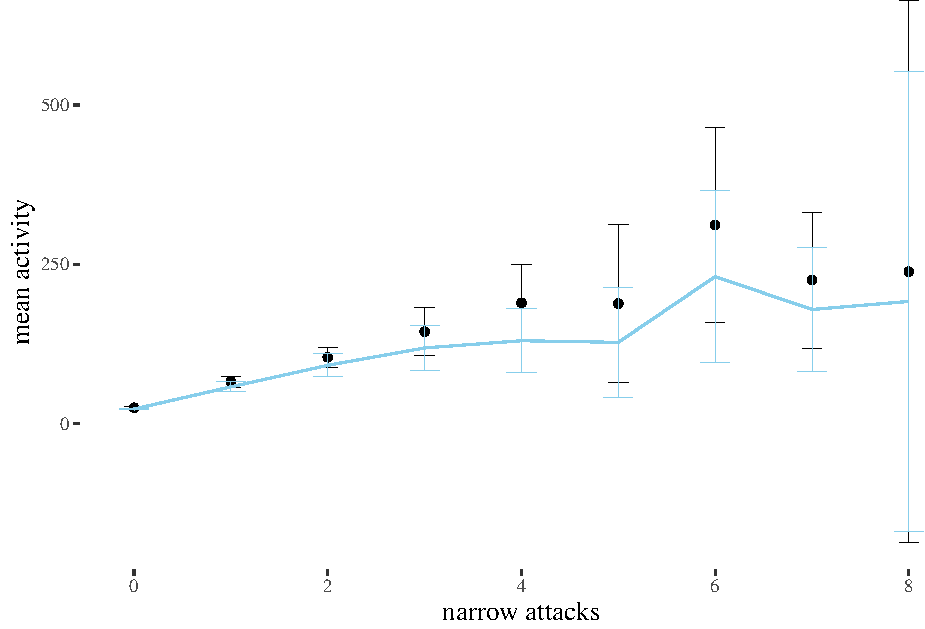
\includegraphics[width=1\linewidth]{quittingShortAbridgedRevisions3_files/figure-latex/unnamed-chunk-60-1} \end{center}
\caption{Mean activity before (black) with 95\% CI error bars and after (blue) , grouped by the number of narrow attacks.}
\end{figure}

Spearman correlation between the distance from the mean and the activity
change is -0.269, which is fairly weak. Pearson's \(\rho\) is not very
different ( -0.255), but we need to be careful here, because the
relation doesn't seem very linear (\(p\)-values for correlation tests
are both \(<0.001\)). If, however, we follow this line of reasoning, the
distance from the mean would explain only \(R^2 =\) 0.065 of the
variability in the activity change in the control group.

The impression of regression to the mean disappears when we look at
\textsf{activityScore}, that is, activity change in proportion to
previous activity (Fig. \ref{fig:regression2}).

\begin{figure}[H]

\begin{center}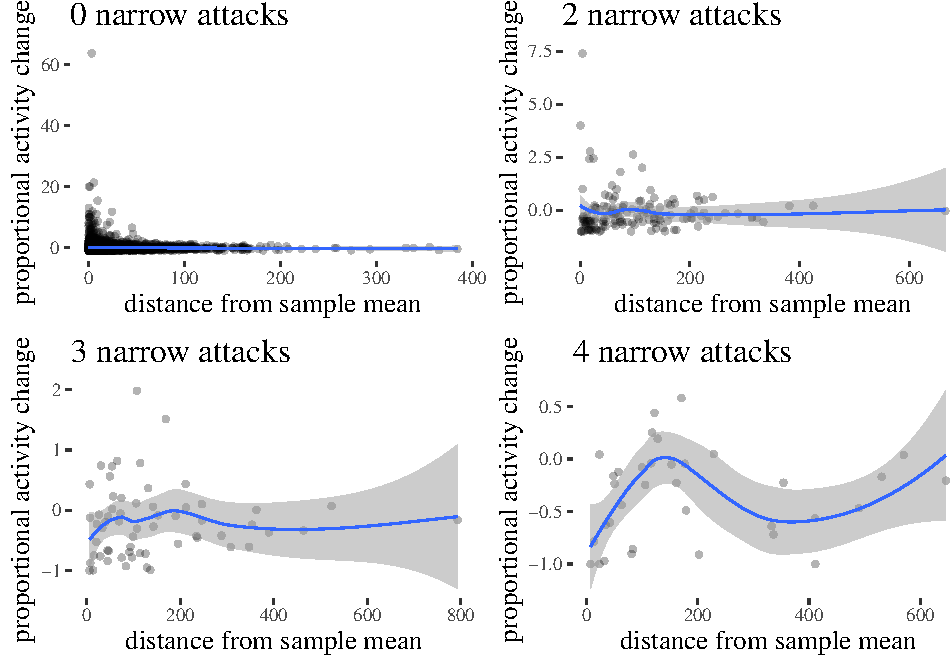
\includegraphics[width=1\linewidth]{quittingShortAbridgedRevisions3_files/figure-latex/unnamed-chunk-61-1} \end{center}
\caption{Distance from sample mean vs. activity score, grouped by the number of attacks (plot for 1 narrow attack omitted, as it is visually not too distinct from the one for 0 attacks).}
\label{fig:regression2}
\end{figure}

Plots for \(>0\) attacks with gam smoothing does not suggest regression
to the mean: it is not the case that attacked users with higher activity
before indeed tend to have lower activity in the second week.

Next, notice that restricting the dataset to users with similar activity
before still results in uneven activity change between the groups. We
focus focus on users with \textsf{activityBefore} restricted to the
third quartile of the whole sample (44), narrow attacks in \$\{0,1,2,3,
4\} and estimate their \textsf{activityScore} proportional drop.

\normalsize

The estimated means of proportional changes are
\(0.05, 0.11, -0.09,-0.35, -0.7\) with decreasing p-values falling below
.05 at the number of attacks \(=3, 4\) and \(p\)-value 0.002 for four
attacks (that is, 0.01 with Bonferroni correction for multiple testing),
despite the group sizes for three and four attacks being fairly low (49
for two, 13 for three, 7 for four). By the way, note that with this
activity restriction, receiving one attack does not seem to have much
impact on user's activity.

\begin{table}[H]
\footnotesize
\scalebox{0.8}{

\begin{tabular}{l|r|r|r|r|l|r}
\hline
Effect & DFn & DFd & F & p & p<.05 & ges\\
\hline
activityBefore & 1 & 3651 & 577.220 & 0 & * & 0.137\\
\hline
fhigh & 20 & 3651 & 10.214 & 0 & * & 0.053\\
\hline
\end{tabular}
}
\normalsize 
\caption{Results of ANCOVA test of activity difference vs. activity before and the number of narrow attacks received.}
\end{table}

Further, to adjust for regression to the mean, it is sometimes
recommended to use ANCOVA to correct for prior differences in pretest
measurements.

\noindent In our case, a statistically significant difference for
different number of attacks received remains after correcting for
differences in activity before.

Finally, the model-theoretic analysis already corrects for activity
before, and estimates the effect size of the other variables keeping
activity before fixed at the mean level. So, regression to the mean,
while it might play a small part, does not seem to explain the
differences. However, the potential effects of regression to the mean
have to be kept in mind in future observational studies and replication
attempts.

One reason this somewhat extensive discussion of regression to the mean
was needed was our group selection method. Perhaps, one could argue, it
would be better to simply randomly pick users and track their fate
starting at some particular time. This way, perhaps, we could avoid
uneven activity levels in the first week between the groups. Attacks are
fairly rare so it quite likely that users receiving attacks during the
observation period would still be the more active ones. Moreover, due to
the rarity of attacks, by proceeding this way and collecting data for
two weeks only we would run a risk of ending up with very small
treatment groups, which could render the data useless. However in our
planned long-term experiment such a risk is much lower, and we will
attempt to replicate our initial results presented in this paper using a
different data collection method.

Another problem that should be mentioned is the population bias, due to
which the results might not be generalizable to populations from other
social networking sites. As of 2018, Reddit had 330 million monthly
active users
\footnote{\url{https://mediakix.com/blog/reddit-statistics-users-demographics/}},
out of which 54\% come from the U.S., 8\% from the UK, and 6.4\% from
Canada. 69\% of its users are male. It's also popular among young adults
--- people between the ages of 25-34 make up around 45\% of the user
base. This is quite a different population than, for instance, the one
using Instagram (with the majority of females and users outside of the
U.S.\footnote{\url{https://www.omnicoreagency.com/instagram-statistics/}}).

Although models created by Samurai Labs mitigate some existing pitfalls
in cyberviolence detection (high false alarm rates), they are not
without flaws. Optimizing for precision can lead to the reduction of
recall. Some attacks that occurred during the data collection period
could be undetected --- the control group could have received messages
expressing verbal aggression that were not included in the analysis,
because they fell outside of the scope of model detection. Also, models
were designed to detect online violence only in English. Attacks
expressed in languages other than English would not get detected either.

\subsection{Causal interpretation}

Clearly, the results are correlational. The question arises: to what
extent do they justify a causal interpretation, according to which
receiving personal attacks causes users to be less active? We believe it
useful to discuss the result in light of the Bardford Hill criteria for
causal inference (Hill, 1965), which are fairly commonly in use in
epidemiological studies (Lucas \& McMichael, 2005), in a slightly
modified up-to-date form (Howick, Glasziou, \& Aronson, 2009) (see
however, for instance, (Pearl \& Mackenzie, 2018) for an insightful
skeptical stance towards these criteria).

So here's the usual list of criteria whose satisfaction tends to justify
the causal interpretation of results, together with our discussion of
how they relate to our study.

\vspace{2mm}

\begin{description}
\item \textbf{Direct evidence.} Here, a few points need to be considered:
\begin{description}
\item The effect should \textbf{not be attributable to plausible confounding factors}.  

\textbf{Comment.} We have already discussed confounding factors. At present, we are not aware of plausible confounding factors. If there are any, they are yet to be discovered.


\item \textbf{Appropriate temporal and/or spatial proximity.}


\textbf{Comment.} Given the nature of the phenomenon, spatial proximity is not relevant. The temporal proximity condition is satisfied: we investigated the activity change within a few days after the attacks.




\item \textbf{Dose responsivenes and reversibility.}


\textbf{Comment.} For those numbers of attacks for which the group sizes allowed for a decent power of statistical tests (see our discussion of power in the section on classical analysis), it seems that the activity drop is responsive to the number of attacks received. For higher numbers of attacks, we have insufficient data. Attention needs to be paid to dose responsiveness in a planned long-term study which is likely to collect sufficient data for higher numbers of attacks. Studies on reversibility are yet to be performed and are not easy to design given that there is no clear way of de-offending users.



\end{description}


\item \textbf{Mechanistic evidence.} A plausible mechanism underlying the correlation should not be absent, and preferably the posed mechanism should be supported by independent considerations (\textbf{coherence} with what is currently known).

\textbf{Comment.} The posed mechanism is not too surprising. People, when they receive personal attacks, are less eager to try to communicate, especially to limit the risk of further attacks.  Various forms of verbal aggression such as cyberbullying have been shown to lead to depression, feeling of hopelessness or powerlessness, as well as can contribute to the so-called social media fatigue ---  which can be characterized by  overall exhaustion, distress, and discontinued intention to use. This in turn can be reflected at a behavioral level --- users who receive an attack might post less in order to avoid yet another attack.



\item \textbf{Parallel evidence.} The study should be replicated, and there should be similar studies showing analogous effects. 


\textbf{Comment.} This is a new result, but we plan to test the models obtained in this study on future data, and to perform a long-term study, where part of the data will be used in a replication attempt. However, several studies have already examined the psychological effects as well as the declared actions undertaken by the victims of the attacks. People who fell victim to online harassment or cyberbullying, often  declared leaving or temporarily stopping the use of an internet service as a result of an attack. 




\end{description}

\section{Discussion: potential solutions to personal attacks, verbal aggression and hate speech}
\label{discussion}

A number of studies have investigated potential means to mitigate social
network depopulation caused by personal attacks and other forms of
online harassment, with almost all of them pointing to the importance of
\textit{efficient moderation}.

One of the strategies that can serve as a potentially effective way to
curb verbal abuse is counter-speech. As shown in (Munger, 2017) it can
lead to a significant reduction of the number of racist tweets, but
also, according to Miškolci, Kováčová, \& Rigová (2020), can encourage
bystander interventions in the form of expressing pro-minority attitude.
In a quasi-experimental research design they have used two argumentative
strategies: fact-checking and/or personal experience under the posts of
politicians' posts from Slovakia related to the topic of the Roma. They
found out that when new users entered Facebook discussions with pro-Roma
comments, it motivated other followers to join the discussion arguing in
favor of the Roma as well.

Johnson et al. (2019) proposed a set of policies and interventions based
on the mathematical understanding of the online hate dynamics that
happen on a cross-platform scale, and found out that ``using entirely
public data from different social media platforms, countries and
languages, (\dots) online hate thrives globally through self-organized,
mesoscale clusters that interconnect to form a resilient
network-of-networks of hate highways across platforms, countries and
languages.''

According to the first proposed policy, reduction of such hate clusters
should stem from banning smaller clusters in the first place (banning
large clusters first could not yield the desired results, as others of
similar size would quickly replace them). According to the second
policy, platforms should randomly ban a small fraction of individual
users across the online hate population. The reasoning behind this
policy was that "choosing a small fraction lowers the risk of multiple
lawsuits, and choosing randomly serves the dual role of lowering the
risk of banning many from the same cluster, and inciting a large crowd.
In the third policy they proposed juxtaposing hate clusters with
anti-hate users and communities, as this way hate-cluster can be
neutralized with the number of determined anti-hate users.

Moreover, simply by displaying the rules, thus making community norms
more visible and accessible to all users, Matias (2019) increased
newcomer rule compliance by 8 percentage points and increased the
participation rate of newcomers in discussions by 70 percent on average
of the communities existing on Reddit --- r/science. Thus making the
rules visible and accessible influenced how people behaved online and
who chose to join.

The efficacy of moderation, usually in its extreme forms, such as
banning users from SNS or even banning whole SNS channels, was also
analyzed in the literature, especially by Chandrasekharan et al. (2017).
They analyzed over hundred million of Reddit posts related to a ban of
two Reddit channels (r/fatpeoplehate and r/CoonTown) due to massive
violations of Reddit's anti-harassment policy (e.g., hate speech against
obese people), and noticed, that an overwhelming majority (more than
eighty percent of users) stopped hate speech-related activities
whatsoever after the ban. Although the measures taken by Reddit to solve
the problem were extreme, this suggests that similar strong statements
by the moderators could be effective also for other forms of bullying
and hate-speech. The efficacy of such ``chilling effects,'' also with
regards to more general and non-directed actions such as implementation
and dissemination of laws, regulations, and policies, or state actions
like surveillance, was also pointed out by Penney (2017).

When it comes to a local moderation, especially on the user-end side,
Navarro, Clevenger, Beasley, \& Jackson (2017) highlight the importance
of ``guardianship'' in, particularly young and adolescent users, and
point out that at present the cyberspace lacks any form of effective
guardianship. Although by guardianship they mainly mean parents and
caregivers of the young users, who should be proactively involved in
educating, monitoring the activity and solving problems occurring to
their kids online, they also acknowledge that this is difficult to
achieve globally and point out that it is also necessary to investigate
other, more effective and efficient forms of guardianship within SNS.
However, as methods of guardianship based purely on low-level
technological solutions, such as filters and software programs were
previously found ineffective (Navarro \& Jasinski, 2012, 2013), the need
for a combined effort becomes apparent, in which specially designated
guardians, such as SNS group and channel moderators, are supported with
more sophisticated technology, such as Artificial Intelligence-based
methods for the detection of personal attacks.

Another study highlighting the role of moderators for the growth of
social networks was done by Seering, Wang, Yoon, \& Kaufman (2019). In
their study, involving in-depth interviews with fifty six moderators
from Twitch, Reddit and Facebook, they conclude that, although it is
more effective to have human moderators than purely algorithmic ones, it
is crucial to ``develop and improve tools that allow moderators to focus
their attention where it is needed.'' In particular, this involves the
development of tools providing ``predictive suggestions for threads or
discussions that might soon devolve.'' Such tools, combined with
user-controlled tools, such as attaching red flags to harmful messages,
would be useful as complementary measures. Seering, Wang, Yoon, \&
Kaufman (2019) point out that moderators are an important part of each
social network, who help the communities grow, evolve, and become
meaningful for its users and thus should be supported in their work for
the constant improvement of social media.

\section{Conclusions and future work}
\label{conclusions}

In this paper we introduced our study on the effects of personal attacks
on users' engagement and continuation of activity in social media.
Despite of the existence of a vast literature on this topic, the
previous works were small-scale (up to several hundred subjects), and
were based on self-reporting. With the growing importance of social
networking services (SNS) in many people's lives, and with the quickly
growing number of online harassment and cyberbullying cases world-wide,
there is a clear need for more direct and quantitative research.
Therefore, we performed a multifaceted quantitative analysis of how the
activity of users subjected to personal attacks changes after
experiencing the attack. To perform the study we applied a
high-precision personal attack detection tool \textsf{Samurai,} to a
fairly large dataset from Reddit, a popular social media platform. The
result was subjected to statistical analysis. The results of our study,
based on several hundred thousand posts and comments clearly showed that
the activity of users experiencing personal attacks online deteriorates
fairly quickly even after one attack. It is not know whether and to what
extent attacked users regain their activity --- this needs further
research --- but even temporarily frequent exposure to personal attacks
will cause disengagement with the platform and arguably lead to its
depopulation.

The negative impact of personal attacks and the mitigating role of
moderation jointly suggest that it is in the best interest of SNS
providers to efficiently detect and moderate personal attacks and
similar cases of harassment and cyberbullying. Moreover, since the
reality of information explosion we live today makes it impossible to
detect and moderate all of such harmful content manually, it becomes
clear that supportive tools, such as the one applied in this research
will become more and more necessary for this purpose.

The literature we discussed provides clear directions to improve social
media experience across platforms, by assuring a sufficient number of
moderators necessarily supported with sophisticated predictive
technologies (such as AI-based tools for automatic cyberbullying
detection) empowering the moderators in their work, and making it less
stressful and more efficient.

Observe also that (Chandrasekharan et al., 2017) (and also (Pudipeddi,
Akoglu, \& Tong, 2014), though on a much smaller scale) were the only
studies among the ones we surveyed that performed a large scale
quantitative analysis, and not self-report-based studies. This shows the
urgent need for similar studies based on a methodology of large scale
quantitative analysis, such as the one we presented. These are important
for a conceptual replication of small scale survey-based qualitative
studies, and become possible thanks to the development of AI-based tools
such as the one used in our study.

In the near future we plan to perform a more long-term study on the same
social media platform (Reddit) to investigate the impact personal
attacks have in a longer perspective, and how they are related to users
completely abandoning the use. This will give us a clear yellow- and
red-alert threshold methods useful for SNS providers to triage their
moderation efforts in case of being flooded with reports. Another
examination will be based on psycholinguistic and other types of
features of users' comments before and after the attacks were received.
As we suspect, there might be a difference not only in the frequency of
comments being posted but also in its characteristics (e.g.~topic,
sentiment, etc.).
\todo{new - added to future work, perhaps to check whether it makes sense}

We also plan to study situations in which the users have not only
regained their activity levels, but their situation improved leading to
an even greater engagement. From our research so far, based on anecdotal
examples found in the analyzed dataset, we can suspect that such
situations are possible, but for them to take place a helping and
proactive activity from other users is necessary, e.g., when a number of
users support the victim and oppose the attacker. Moreover, we noticed
that when other users are capable of mitigating the conflict, especially
with empathetic engagement, it is possible to not only help the victim,
but also resolve the conflict, which is the optimal way the events can
unfold. Not only from the point of view of all the sides of the
conflict, but also from the perspective of the SNS providers, as keeping
the health of SNS platform in good shape is crucial to assure its
sustainable growth and stop depopulation.

Apart from the above, we plan to continue the study on other SNS
platforms, including Twitter, Facebook, or Instagram, also in languages
other than English, such as Polish and Japanese. Finally, we plan to
expand the functionalities of the \textsf{ Samurai} system to cover
various types of attacks, including other types of harassment (sexual,
racial, child abuse, etc.), as well as focus not only on detecting the
attacks, but also on the victims' situation, and develop models for
detecting suicidal intent in users' messages, to contribute to the
improvement of the general health of social media and its users.

\newpage

\section*{References}

\hypertarget{refs}{}
\begin{CSLReferences}{1}{0}
\leavevmode\hypertarget{ref-Akaike1974model}{}%
Akaike, H. (1974). A new look at the statistical model identification.
\emph{IEEE Transactions on Automatic Control}, \emph{19}(6), 716--723.
\url{https://doi.org/10.1109/TAC.1974.1100705}

\leavevmode\hypertarget{ref-andersen2001satiation}{}%
Andersen, E. S. (2001). Satiation in an evolutionary model of structural
economic dynamics. In \emph{Escaping satiation} (pp. 165--186).
Springer. \url{https://doi.org/10.1007/978-3-662-04528-2_10}

\leavevmode\hypertarget{ref-arguello2006talk}{}%
Arguello, J., Butler, B. S., Joyce, E., Kraut, R., Ling, K. S., Rosé,
C., \& Wang, X. (2006). Talk to me: Foundations for successful
individual-group interactions in online communities. \emph{Proceedings
of the SIGCHI Conference on Human Factors in Computing Systems},
959--968. \url{https://doi.org/10.1145/1124772.1124916}

\leavevmode\hypertarget{ref-barlett2015anonymously}{}%
Barlett, C. P. (2015). Anonymously hurting others online: The effect of
anonymity on cyberbullying frequency. \emph{Psychology of Popular Media
Culture}, \emph{4}(2), 70. \url{https://doi.org/10.1037/a0034335}

\leavevmode\hypertarget{ref-barlett2016predicting}{}%
Barlett, C. P., Gentile, D. A., \& Chew, C. (2016). Predicting
cyberbullying from anonymity. \emph{Psychology of Popular Media
Culture}, \emph{5}(2), 171. \url{https://doi.org/10.1037/ppm0000055}

\leavevmode\hypertarget{ref-barlinska2018slowami}{}%
Barlińska, J., Plichta, P., Pyżalski, J., \& Szuster, A. (2018). Ich
s{ł}owami---obraz pomocy w sytuacjach cyberprzemocy r{ó}wie{ś}niczej z
perspektywy uczni{ó}w. \emph{Dziecko Krzywdzone. Teoria, Badania,
Praktyka}, \emph{17}(4), 82--115.

\leavevmode\hypertarget{ref-beran2005cyber}{}%
Beran, T., \& Li, Q. (2005). Cyber-harassment: A study of a new method
for an old behavior. \emph{Journal of Educational Computing Research},
\emph{32}(3), 265.

\leavevmode\hypertarget{ref-bilewicz2020hate}{}%
Bilewicz, M., \& Soral, W. (2020). Hate speech epidemic. The dynamic
effects of derogatory language on intergroup relations and political
radicalization. \emph{Political Psychology}.
\url{https://doi.org/10.1111/pops.12670}

\leavevmode\hypertarget{ref-campbell2012victims}{}%
Campbell, M., Spears, B., Slee, P., Butler, D., \& Kift, S. (2012).
Victims' perceptions of traditional and cyberbullying, and the
psychosocial correlates of their victimisation. \emph{Emotional and
Behavioural Difficulties}, \emph{17}(3-4), 389--401.
\url{https://doi.org/10.1080/13632752.2012.704316}

\leavevmode\hypertarget{ref-cao2019consequences}{}%
Cao, X., Khan, A. N., Ali, A., \& Khan, N. A. (2019). Consequences of
cyberbullying and social overload while using {SNSs}: A study of users'
discontinuous usage behavior in {SNSs}. \emph{Information Systems
Frontiers}, 1--14. \url{https://doi.org/10.1007/s10796-019-09936-8}

\leavevmode\hypertarget{ref-carey2016influences}{}%
Carey, M. C., \& Meyer, H. K. (2016). The influences of participation
and moderation on the development of a sense of virtual community.
\emph{International Journal of Web Based Communities}, \emph{12}(4),
326--341. \url{https://doi.org/10.1504/ijwbc.2016.080812}

\leavevmode\hypertarget{ref-chandrasekharan2017you}{}%
Chandrasekharan, E., Pavalanathan, U., Srinivasan, A., Glynn, A.,
Eisenstein, J., \& Gilbert, E. (2017). You can't stay here: The efficacy
of {R}eddit's 2015 ban examined through hate speech. \emph{Proceedings
of the ACM on Human-Computer Interaction}, \emph{1}(CSCW), 1--22.

\leavevmode\hypertarget{ref-chua2019understanding}{}%
Chua, Y. T. (2019). \emph{Understanding radicalization process in online
far-right extremist forums using social influence model}. Michigan State
University.

\leavevmode\hypertarget{ref-cross2012virtual}{}%
Cross, E., Piggin, R., Douglas, T., \& Vonkaenel-Flatt, J. (2012).
Virtual violence {II}: Progress and challenges in the fight against
cyberbullying. \emph{London: Beatbullying}.

\leavevmode\hypertarget{ref-culpepperexploring}{}%
Culpepper, M. (2020). \emph{Exploring the relationships of social media
usage and symptoms of anxiety and depression in adolescents}. Abilene
Christian University.

\leavevmode\hypertarget{ref-cvijikj2013online}{}%
Cvijikj, I. P., \& Michahelles, F. (2013). Online engagement factors on
{F}acebook brand pages. \emph{Social Network Analysis and Mining},
\emph{3}(4), 843--861. \url{https://doi.org/10.1007/s13278-013-0098-8}

\leavevmode\hypertarget{ref-de2008stormfront}{}%
De Koster, W., \& Houtman, D. (2008). {`STORMFRONT IS LIKE a SECOND HOME
TO ME'} on virtual community formation by right-wing extremists.
\emph{Information, Communication \& Society}, \emph{11}(8), 1155--1176.
\url{https://doi.org/10.1080/13691180802266665}

\leavevmode\hypertarget{ref-hamilton2017loyalty}{}%
Hamilton, W. L., Zhang, J., Danescu-Niculescu-Mizil, C., Jurafsky, D.,
\& Leskovec, J. (2017). Loyalty in online communities. \emph{Proceedings
of the International {AAAI Conference on Weblogs and Social Media}},
\emph{2017}, 540. NIH Public Access.

\leavevmode\hypertarget{ref-hill1965environment}{}%
Hill, A. B. (1965). \emph{The environment and disease: Association or
causation?} Sage Publications.
\url{https://doi.org/10.1177/003591576505800503}

\leavevmode\hypertarget{ref-hinduja2008cyberbullying}{}%
Hinduja, S., \& Patchin, J. W. (2008). Cyberbullying: An exploratory
analysis of factors related to offending and victimization.
\emph{Deviant Behavior}, \emph{29}(2), 129--156.
\url{https://doi.org/10.1080/01639620701457816}

\leavevmode\hypertarget{ref-howick2009evolution}{}%
Howick, J., Glasziou, P., \& Aronson, J. K. (2009). The evolution of
evidence hierarchies: What can {Bradford Hill's} `guidelines for
causation'contribute? \emph{Journal of the Royal Society of Medicine},
\emph{102}(5), 186--194.

\leavevmode\hypertarget{ref-johnson2019hidden}{}%
Johnson, N., Leahy, R., Restrepo, N., Johnson, Velasquez, N., Zheng, M.,
\ldots{} Wuchty, S. (2019). Hidden resilience and adaptive dynamics of
the global online hate ecology. \emph{Nature}, \emph{573}(7773),
261--265. \url{https://doi.org/10.1038/s41586-019-1494-7}

\leavevmode\hypertarget{ref-kelly2018social}{}%
Kelly, Y., Zilanawala, A., Booker, C., \& Sacker, A. (2018). Social
media use and adolescent mental health: Findings from the UK millennium
cohort study. \emph{EClinicalMedicine}, \emph{6}, 59--68.
\url{https://doi.org/10.1016/j.eclinm.2018.12.005}

\leavevmode\hypertarget{ref-kircaburun2016self}{}%
Kircaburun, K. (2016). Self-esteem, daily {I}nternet use and social
media addiction as predictors of depression among {T}urkish adolescents.
\emph{Journal of Education and Practice}, \emph{7}(24), 64--72.

\leavevmode\hypertarget{ref-kitazawa2018associations}{}%
Kitazawa, M., Yoshimura, M., Murata, M., Sato-Fujimoto, Y., Hitokoto,
H., Mimura, M., \ldots{} Kishimoto, T. (2018). Associations between
problematic internet use and psychiatric symptoms among university
students in {J}apan. \emph{Psychiatry and Clinical Neurosciences},
\emph{72}(7), 531--539. \url{https://doi.org/10.1111/pcn.12662}

\leavevmode\hypertarget{ref-Kruschke2015}{}%
Kruschke, J. K. (2015). \emph{Doing {B}ayesian data analysis; a tutorial
with {r}, {JAGS}, and {stan}}.

\leavevmode\hypertarget{ref-lampe2014crowdsourcing}{}%
Lampe, C., Zube, P., Lee, J., Park, C. H., \& Johnston, E. (2014).
Crowdsourcing civility: A natural experiment examining the effects of
distributed moderation in online forums. \emph{Government Information
Quarterly}, \emph{31}(2), 317--326.
\url{https://doi.org/10.1016/j.giq.2013.11.005}

\leavevmode\hypertarget{ref-lemmens2020managing}{}%
Lemmens, A., \& Gupta, S. (2020). Managing churn to maximize profits.
\emph{Marketing Science, Forthcoming}.
\url{https://doi.org/10.2139/ssrn.2964906}

\leavevmode\hypertarget{ref-lucas2005association}{}%
Lucas, R. M., \& McMichael, A. J. (2005). Association or causation:
Evaluating links between "environment and disease". \emph{Bulletin of
the World Health Organization}, \emph{83}, 792--795.

\leavevmode\hypertarget{ref-malik2020correlates}{}%
Malik, A., Dhir, A., Kaur, P., \& Johri, A. (2020). Correlates of social
media fatigue and academic performance decrement. \emph{Information
Technology \& People}. \url{https://doi.org/10.1108/itp-06-2019-0289}

\leavevmode\hypertarget{ref-mathew2019temporal}{}%
Mathew, B., Illendula, A., Saha, P., Sarkar, S., Goyal, P., \&
Mukherjee, A. (2019). Temporal effects of unmoderated hate speech in
gab. \emph{arXiv Preprint arXiv:1909.10966}.

\leavevmode\hypertarget{ref-matias2019preventing}{}%
Matias, J. N. (2019). Preventing harassment and increasing group
participation through social norms in 2,190 online science discussions.
\emph{Proceedings of the National Academy of Sciences}, \emph{116}(20),
9785--9789. \url{https://doi.org/10.1073/pnas.1813486116}

\leavevmode\hypertarget{ref-meyer2014moderation}{}%
Meyer, H. K., \& Carey, M. C. (2014). In moderation: Examining how
journalists' attitudes toward online comments affect the creation of
community. \emph{Journalism Practice}, \emph{8}(2), 213--228.
\url{https://doi.org/10.1080/17512786.2013.859838}

\leavevmode\hypertarget{ref-mivskolci2020countering}{}%
Miškolci, J., Kováčová, L., \& Rigová, E. (2020). Countering hate speech
on {F}acebook: The case of the {R}oma minority in {S}lovakia.
\emph{Social Science Computer Review}, \emph{38}(2), 128--146.
\url{https://doi.org/10.1177/0894439318791786}

\leavevmode\hypertarget{ref-mohan2017impact}{}%
Mohan, S., Guha, A., Harris, M., Popowich, F., Schuster, A., \& Priebe,
C. (2017). The impact of toxic language on the health of {R}eddit
communities. \emph{Canadian Conference on Artificial Intelligence},
51--56. Springer. \url{https://doi.org/10.1007/978-3-319-57351-9_6}

\leavevmode\hypertarget{ref-munger2017tweetment}{}%
Munger, K. (2017). Tweetment effects on the tweeted: Experimentally
reducing racist harassment. \emph{Political Behavior}, \emph{39}(3),
629--649. \url{https://doi.org/10.1007/s11109-016-9373-5}

\leavevmode\hypertarget{ref-navarro2017one}{}%
Navarro, J. N., Clevenger, S., Beasley, M. E., \& Jackson, L. K. (2017).
One step forward, two steps back: Cyberbullying within social networking
sites. \emph{Security Journal}, \emph{30}(3), 844--858.
\url{https://doi.org/10.1057/sj.2015.19}

\leavevmode\hypertarget{ref-navarro2012going}{}%
Navarro, J. N., \& Jasinski, J. L. (2012). Going cyber: Using routine
activities theory to predict cyberbullying experiences.
\emph{Sociological Spectrum}, \emph{32}(1), 81--94.
\url{https://doi.org/10.1080/02732173.2012.628560}

\leavevmode\hypertarget{ref-navarro2013girls}{}%
Navarro, J. N., \& Jasinski, J. L. (2013). Why girls? Using routine
activities theory to predict cyberbullying experiences between girls and
boys. \emph{Women \& Criminal Justice}, \emph{23}(4), 286--303.
\url{https://doi.org/10.1080/08974454.2013.784225}

\leavevmode\hypertarget{ref-nasi2014association}{}%
Näsi, M., Räsänen, P., Oksanen, A., Hawdon, J., Keipi, T., \& Holkeri,
E. (2014). Association between online harassment and exposure to harmful
online content: A cross-national comparison between the united states
and finland. \emph{Computers in Human Behavior}, \emph{41}, 137--145.
\url{https://doi.org/10.1016/j.chb.2014.09.019}

\leavevmode\hypertarget{ref-nixon2014current}{}%
Nixon, C. L. (2014). Current perspectives: The impact of cyberbullying
on adolescent health. \emph{Adolescent Health, Medicine and
Therapeutics}, \emph{5}, 143. \url{https://doi.org/10.2147/ahmt.s36456}

\leavevmode\hypertarget{ref-ortiz2019rise}{}%
Ortiz-Ospina, E. (2019). The rise of social media. \emph{Our World in
Data}, \emph{18}. Retrieved from
\url{https://ourworldindata.org/rise-of-social-media}

\leavevmode\hypertarget{ref-pearl2018why}{}%
Pearl, J., \& Mackenzie, D. (2018). \emph{The book of why: The new
science of cause and effect} (1st ed.). USA: Basic Books, Inc.
\url{https://doi.org/10.1080/01621459.2020.1721245}

\leavevmode\hypertarget{ref-penney2017internet}{}%
Penney, J. W. (2017). Internet surveillance, regulation, and chilling
effects online: A comparative case study. \emph{Internet Policy Review},
\emph{6}(2). \url{https://doi.org/10.14763/2017.2.692}

\leavevmode\hypertarget{ref-preece2004top}{}%
Preece, J., Nonnecke, B., \& Andrews, D. (2004). The top five reasons
for lurking: Improving community experiences for everyone.
\emph{Computers in Human Behavior}, \emph{20}(2), 201--223.
\url{https://doi.org/10.1016/j.chb.2003.10.015}

\leavevmode\hypertarget{ref-ptaszynski2018automatic}{}%
Ptaszynski, M. E., \& Masui, F. (2018). \emph{Automatic cyberbullying
detection: Emerging research and opportunities: Emerging research and
opportunities}. IGI Global.

\leavevmode\hypertarget{ref-ptaszynski2018cyberbullying}{}%
Ptaszyński, M., Leliwa, G., Piech, M., \& Smywiński-Pohl, A. (2018).
Cyberbullying detection--technical report 2/2018, {Department of
Computer Science AGH, University of Science and Technology}. \emph{arXiv
Preprint arXiv:1808.00926}.

\leavevmode\hypertarget{ref-pudipeddi2014user}{}%
Pudipeddi, J. S., Akoglu, L., \& Tong, H. (2014). User churn in focused
question answering sites: Characterizations and prediction.
\emph{Proceedings of the 23rd International Conference on World Wide
Web}, 469--474. \url{https://doi.org/10.1145/2567948.2576965}

\leavevmode\hypertarget{ref-pyzalski2019polish}{}%
Pyżalski, J., Zdrodowska, A., Tomczyk, Ł., \& Abramczuk, K. (2019).
Polish research {EU KIDS ONLINE}. The most important results and
conclusions. \emph{Pozna{ń}: Wydaw. Uniwersytet Adama Mickiewicza}.

\leavevmode\hypertarget{ref-raskauskas2007involvement}{}%
Raskauskas, J., \& Stoltz, A. D. (2007). Involvement in traditional and
electronic bullying among adolescents. \emph{Developmental Psychology},
\emph{43}(3), 564. \url{https://doi.org/10.1037/0012-1649.43.3.564}

\leavevmode\hypertarget{ref-raub2015phenomenological}{}%
Raub, K. (2015). \emph{A phenomenological inquiry into {F}acebook
newcomer motivations for participatory activities} (PhD thesis). Nova
Southeastern University.

\leavevmode\hypertarget{ref-rosner2016dangerous}{}%
Rösner, L., Winter, S., \& Krämer, N. C. (2016). Dangerous minds?
Effects of uncivil online comments on aggressive cognitions, emotions,
and behavior. \emph{Computers in Human Behavior}, \emph{58}, 461--470.
\url{https://doi.org/10.1016/j.chb.2016.01.022}

\leavevmode\hypertarget{ref-sadeque2019predicting}{}%
Sadeque, F., \& Bethard, S. (2019). Predicting engagement in online
social networks: Challenges and opportunities. \emph{arXiv Preprint
arXiv:1907.05442}.

\leavevmode\hypertarget{ref-saiphoo2020social}{}%
Saiphoo, A. N., Halevi, L. D., \& Vahedi, Z. (2020). Social networking
site use and self-esteem: A meta-analytic review. \emph{Personality and
Individual Differences}, \emph{153}, 109639.
\url{https://doi.org/10.1016/j.paid.2019.109639}

\leavevmode\hypertarget{ref-savimaki2020disquieted}{}%
Savimäki, T., Kaakinen, M., Räsänen, P., \& Oksanen, A. (2020).
Disquieted by online hate: Negative experiences of finnish adolescents
and young adults. \emph{European Journal on Criminal Policy and
Research}, \emph{26}(1), 23--37.
\url{https://doi.org/10.1007/s10610-018-9393-2}

\leavevmode\hypertarget{ref-seering2019moderator}{}%
Seering, J., Wang, T., Yoon, J., \& Kaufman, G. (2019). Moderator
engagement and community development in the age of algorithms. \emph{New
Media \& Society}, \emph{21}(7), 1417--1443.
\url{https://doi.org/10.1177/1461444818821316}

\leavevmode\hypertarget{ref-sheth2020borderless}{}%
Sheth, J. N. (2020). Borderless media: Rethinking international
marketing. \emph{Journal of International Marketing}, \emph{28}(1),
3--12. \url{https://doi.org/10.1177/1069031x19897044}

\leavevmode\hypertarget{ref-sourander2010psychosocial}{}%
Sourander, A., Klomek, A. B., Ikonen, M., Lindroos, J., Luntamo, T.,
Koskelainen, M., \ldots{} Helenius, H. (2010). Psychosocial risk factors
associated with cyberbullying among adolescents: A population-based
study. \emph{Archives of General Psychiatry}, \emph{67}(7), 720--728.
\url{https://doi.org/10.1001/archgenpsychiatry.2010.79}

\leavevmode\hypertarget{ref-Tukey1949}{}%
Tukey, J. W. (1949). Comparing individual means in the analysis of
variance. \emph{Biometrics}, \emph{5}(2), 99.
\url{https://doi.org/10.2307/3001913}

\leavevmode\hypertarget{ref-valkenburg2006friend}{}%
Valkenburg, P. M., Peter, J., \& Schouten, A. P. (2006). Friend
networking sites and their relationship to adolescents' well-being and
social self-esteem. \emph{CyberPsychology \& Behavior}, \emph{9}(5),
584--590. \url{https://doi.org/10.1089/cpb.2006.9.584}

\leavevmode\hypertarget{ref-weber2020online}{}%
Weber, M., Viehmann, C., Ziegele, M., \& Schemer, C. (2020). Online hate
does not stay online--how implicit and explicit attitudes mediate the
effect of civil negativity and hate in user comments on prosocial
behavior. \emph{Computers in Human Behavior}, \emph{104}, 106192.
\url{https://doi.org/10.1016/j.chb.2019.106192}

\leavevmode\hypertarget{ref-williams2020hate}{}%
Williams, M. L., Burnap, P., Javed, A., Liu, H., \& Ozalp, S. (2020).
Hate in the machine: Anti-black and anti-muslim social media posts as
predictors of offline racially and religiously aggravated crime.
\emph{The British Journal of Criminology}, \emph{60}(1), 93--117.
\url{https://doi.org/10.1093/bjc/azz049}

\leavevmode\hypertarget{ref-wise2006moderation}{}%
Wise, K., Hamman, B., \& Thorson, K. (2006). Moderation, response rate,
and message interactivity: Features of online communities and their
effects on intent to participate. \emph{Journal of Computer-Mediated
Communication}, \emph{12}(1), 24--41.
\url{https://doi.org/10.1111/j.1083-6101.2006.00313.x}

\leavevmode\hypertarget{ref-woods2016sleepyteens}{}%
Woods, H. C., \& Scott, H. (2016). \# sleepyteens: Social media use in
adolescence is associated with poor sleep quality, anxiety, depression
and low self-esteem. \emph{Journal of Adolescence}, \emph{51}, 41--49.
\url{https://doi.org/10.1016/j.adolescence.2016.05.008}

\leavevmode\hypertarget{ref-wroczynski2019system}{}%
Wroczynski, M., \& Leliwa, G. (2019). \emph{System and method for
detecting undesirable and potentially harmful online behavior}. Google
Patents.

\leavevmode\hypertarget{ref-ybarra2004linkages}{}%
Ybarra, M. L. (2004). Linkages between depressive symptomatology and
internet harassment among young regular internet users.
\emph{CyberPsychology \& Behavior}, \emph{7}(2), 247--257.
\url{https://doi.org/10.1089/109493104323024500}

\leavevmode\hypertarget{ref-zong2019social}{}%
Zong, W., Yang, J., \& Bao, Z. (2019). Social network fatigue affecting
continuance intention of social networking services. \emph{Data
Technologies and Applications}.
\url{https://doi.org/10.1108/dta-06-2018-0054}

\end{CSLReferences}

\end{document}
